\documentclass[10pt,b5paper,titlepage]{book}

\usepackage[utf8]{inputenc}
\usepackage{amsmath}
\usepackage{amsfonts}
\usepackage{amssymb}
%\usepackage{xcolor}
\usepackage{color}
\usepackage{graphicx}

% python - needs pip install Pygments
\usepackage{minted}
\usemintedstyle{native}

\usepackage{hyperref}

\author{Jan Tomek}
\title{\bf FEM Practices}

% python code format
\setminted[python]{breaklines, framesep=2mm, fontsize=\footnotesize, numbersep=5pt}
\newminted[python]{python}{linenos=true,
                           frame=lines,
                           baselinestretch=1.2,
                           mathescape,
                           xleftmargin=0cm,
                           framesep=2mm,
                           fontsize=\footnotesize}

\setlength{\parindent}{0ex}
\setlength{\parskip}{1em plus 0.1em minus 0.2em}
\renewcommand{\labelitemi}{$\bullet$}
\renewcommand{\labelitemii}{$\bullet$}
\renewcommand{\labelitemiii}{$\bullet$}
\renewcommand{\labelitemiv}{$\bullet$}

%Commands definitions
\newcommand\setbackgroundcolour{\pagecolor[rgb]{0.15,0.15,0.15}}
\newcommand\settextcolour{\color[rgb]{0.9,0.9,0.9}}
\newcommand\invertbackgroundtext{\setbackgroundcolour\settextcolour}

\newcommand*{\Scale}[2][4]{\scalebox{#1}{$#2$}}%
\newcommand*{\Resize}[2]{\resizebox{#1}{!}{$#2$}}%

% equal by definition
\newcommand*\eqd{\stackrel{\triangle}{=}}

% {name}[number of arguments][1st default value] etc..
% the argument value is then inserted at #argument_number
\newenvironment{bbox}[1][0.96]
{
    \begin{center}
        \begin{tabular}{|p{#1\textwidth}|}
            \hline\\
}
{
            \\\\\hline
        \end{tabular}
    \end{center}
}

\newenvironment{bboxtitle}[1][0.96]
{
    \begin{center}
        #1\\[1ex]
        \begin{tabular}{|p{#1\textwidth}|}
            \hline\\
}
{
            \\\\\hline
        \end{tabular}
    \end{center}
}

\newenvironment{eqarray}
{
    \begin{eqnarray}
        \begin{aligned}
}
{
        \end{aligned}
    \end{eqnarray}
}

%Command execution.
%If this line is commented, then the appearance remains as usual.
\invertbackgroundtext

\begin{document}

\maketitle

\tableofcontents

\chapter{Dynamics}

\section{Function properties}

\subsubsection{Sine and Cosine functions}
Let a fucntion $ f(t) $ be in the form:

\begin{equation}
    f(t) = A_1 \cos{\omega t} + B_i \sin{\omega t}
\end{equation}

then the following relation applies:

\begin{eqarray}
    f(t) &= A \cos{\left( \omega t - \phi \right)}\\
    A &= \sqrt{A_1^2 + B_1^2}\\
    \phi &= \tan^{-1} \left( \frac{B_i}{A_i} \right)
\end{eqarray}

also:
\begin{eqarray}
    \cos{\left( \omega t - \phi \right)} &=
    \cos{\omega t} \cos{\phi} + \sin{\omega t} \sin{\phi}\\
    \sin{\left( \omega t - \phi \right)} &=
    \sin{\omega t} \cos{\phi} + \cos{\omega t} \sin{\phi}
\end{eqarray}



\section{SDOF system}

\subsection{Definition}

Let:

\begin{equation}
    m \ddot{u}(t) + c \dot{u}(t) + k u(t) = f(t)
\end{equation}

or:

\begin{equation}
    m a(t) + c v(t) + k u(t) = f(t)
\end{equation}

be the \textbf{SDOF equation of motion}, then the following applies:

\begin{eqarray}
    \omega^2 &= \frac{k}{m} \\
    \omega &= \sqrt{\frac{k}{m}} \\
    f &= \frac{\omega}{2 \pi} \\
    T &= \frac{1}{f}
\end{eqarray}

where:\\
$ \omega $ is radial eigenfrequency [rad/s],\\
$ f $ is eigenfrequency [Hz] and\\
$ T $ is period [s]

The simplest vibratory syslem can be described by a single mass connected to a spring
(and possibly a dashpot). The mass is allowed to travel only along the spring elongation
direction. Such systems are called \textit{Single Degree-of-Freedom} (\textbf{SDOF})
systems and are shown in the figure.

\begin{figure}[ht]
    \centering
    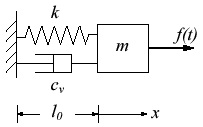
\includegraphics[width=0.90\textwidth]{img/SDOF_plot.png}
    \caption{SDOF system with a linear spring and dashpot}
    \label{fig:SDOF-plot-png}
\end{figure}

\subsection{Equation of Motion for SDOF Systems}

SDOF vibration can be analyzed by \textbf{Newton's second law of motion},
$ F = m a $. The analysis can be easily visualised with the aid of a
\textbf{free body diagram},

\begin{figure}[ht]
    \centering
    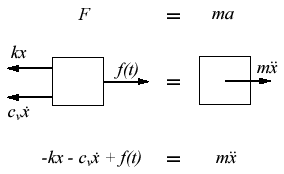
\includegraphics[width=0.90\textwidth]{img/SDOF_FreeBodyDiagram.png}
    \caption{SDOF Free Body Diagram}
    \label{fig:SDOF-freebodydiagram-png}
\end{figure}

The resulting equation of motion is a
\textbf{second order, non-homegeneous, ordinary differential equation}:

\begin{equation}
    m \ddot{u} + c \dot{u} + k u = f(t)
        \left\{ \begin{matrix}
                u(t=0) = u_0\\
                \dot{u}(t=0) = \dot{u}_0
          \end{matrix} \right.
\end{equation}

with the initial conditions $ u_0 $ and $ \dot{u}_0 $.


\subsection{Time Solution for Unforced Undamped SDOF Systems}

\textit{https://www.efunda.com/formulae/vibrations/sdof\_free\_undamped.cfm}

The equation of motion derived in the definition can be simplified to:

\begin{equation}
    m \ddot{u} + k u = 0
        \left\{ \begin{matrix}
                u(t=0) = u_0\\
                \dot{u}(t=0) = \dot{u}_0
          \end{matrix} \right.
\end{equation}

This equation of motion is a
\textbf{second order, homegeneous, ordinary differential equation} (ODE). If the mass
and spring stiffness are constants, the ODE becomes a
\textbf{linear, homogeneous ODE with constant coefficients} and can be solved
by the Characteristic Equation method. The characteristic equation for this
problem is:

\begin{equation}
    m s^2 + k = 0
\end{equation}

which determines the 2 independent roots for the undamped vibration problem.
The final solution (that contains the 2 independent roots from the characteristic
equation and satisfies the initial conditions) is:

\begin{eqarray}
    u(t) &= c_1 e^{i \omega_n t} + c_2 e^{- \omega_n t}\\
         &= d_1 \cos{\omega_n t} + d_2 \sin{\omega_n t} \\
    \implies u(t) &= u_0 \cos{\omega_n t} + \frac{\dot{u}_0}{\omega_n} \sin{\omega_n t}
\end{eqarray}

The natural frequency $ \omega_n $ is defined by:

\begin{equation}
    \omega_n = \sqrt{\frac{k}{m}}
\end{equation}

and depends only on the system mass and the spring stiffness (i.e. any damping will
not change the natural frequency of a system).

Alternatively, the solution may be expressed by the equivalent form,

\begin{equation}
    u(t) = A_0 \cos{(\omega_n t - \phi_0)}
\end{equation}

where the amplitude $ A_0 $ and the intial phase $ \phi_0 $ are given by:

\begin{eqarray}
    A_0 &= \sqrt{u_0^2 + \left(\frac{\dot{u}_0}{\omega_n}\right)^2}\\
    \phi_0 &= \tan^{-1}\frac{\dot{u}_0}{u_0 \omega_n}
\end{eqarray}

\begin{figure}[ht]
    \centering
    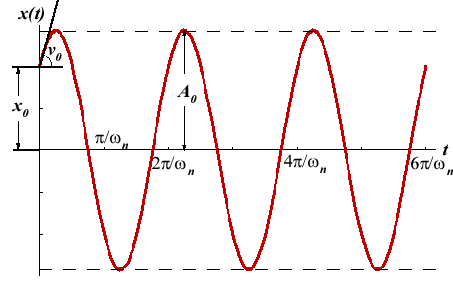
\includegraphics[width=0.90\textwidth]{img/SDOF_Undamped_Response.png}
    \caption{SDOF Undamped sample time behavior}
    \label{fig:SDOF-undamped-response-png}
\end{figure}

Note that an assumption of zero damping is typically not accurate. In reality,
there almost always exists some resistance in vibratory systems. This reistance
will damp the vibration and dissipate energy, the oscillatory motion caused by the
initial disturbance will eventually be reduced to zero.


\subsection{Time Solution for Unforced Damped SDOF Systems}

\textit{https://www.efunda.com/formulae/vibrations/sdof\_free\_damped.cfm}

\begin{figure}[ht]
    \centering
    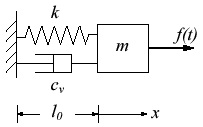
\includegraphics[width=0.90\textwidth]{img/SDOF_plot.png}
    \caption{SDOF system with a linear spring and dashpot}
    \label{fig:SDOF-plot-damped-png}
\end{figure}

Damping that produces a damping force proportional to the mass's velocity is
commonly referred to as \textit{viscous damping}, and is denoted graphically
by a dashpot.

For an unforced damped \textbf{SDOF} system, the general equation of motion
becomes:

\begin{equation}
    m \ddot{u} + c \dot{u} + k u = 0
        \left\{ \begin{matrix}
                u(t=0) = u_0\\
                \dot{u}(t=0) = \dot{u}_0
          \end{matrix} \right.
\end{equation}

Tis equation of motion is a \textbf{second order, homogeneous, ODE}. If all
parameters (mass, stiffness and viscous damping) are constants, the \textbf{ODE}
becomes a \textbf{linear ODE with constant coefficients} and can be solved by
the \textit{Characteristic Equation method}. The characteristic equation for this
problem is:

\begin{equation}
    m s^2 + s_v s + k = 0
\end{equation}

which determines the 2 independent roots for the damped vibration problem.
The roots to the characteristic equation fall into one of the following
3 cases:

\begin{itemize}
    \item If $ c_v^2 - 4 m k < 0 $, the system is termed \textbf{underdamped}.
        The roots of the characteristic equation are complex conjugates,
        corresponding to \textit{oscillatory motion} with an
        \textit{exponential decay} in amplitude.

    \item If $ c_v^2 - 4 m k = 0 $, the system is termed \textbf{critically-derdamped}.
        The roots of the characteristic equation are repeated,
        corresponding to \textit{simple decay motion} with at most
        \textit{one overshoot} of the systems resting position.

    \item If $ c_v^2 - 4 m k > 0 $, the system is termed \textbf{overderdamped}.
        The roots of the characteristic equation are prurely real and distinct,
        corresponding to \textit{simple exponentially decaying motion}.

\end{itemize}

To simplify the solutions coming up, we define the critical damping $ c_c $,
the damping ratio $ \zeta $, and the damped vibration frequency $ \omega_d $ as:

\begin{eqarray}
    c_c &= 2 m \sqrt{\frac{k}{m}} = 2 m \omega_n\\
    \zeta &= \frac{c_v}{c_c}\\
    \omega_d &= \sqrt{1 - \zeta^2} \omega_n
\end{eqarray}

where the natural frequency of the system $ \omega_n $ is given by:

\begin{equation}
    \omega_n = \sqrt{\frac{k}{m}}
\end{equation}

Note that $ \omega_d $ will equal $ \omega_n $ when the damping of the system
is zero (i.e. undamped). The time solutions for the free \textbf{SDOF}
system is presented below for each of the three case scenarios.

\subsubsection{Time Solution of Unforced Underdamped SDOF Systems}

When $ c_v^2 - 4 m k < 0 $ (equivalent to $ \zeta < 1 $ or $ c_v < c_c $),
the characteristic equation has a pair of complex conjugate roots. The displacement
solution for this kind of system is:

\begin{eqarray}
    u(t) &= c_1 e^{-\zeta + i \sqrt{1 - \zeta^2} \omega_n t}
          + c_2 e^{-\zeta - i \sqrt{1 - \zeta^2} \omega_n t}\\
         &= e^{-\zeta \omega_n t} \left[ d_1 \cos{(\omega_d t)}
                                       + d_2 \sin{(\omega_d t)} \right]\\
    \implies u(t) &= \underbrace{e^{-\zeta \omega_n t}}_{exponential\ decay}
    \underbrace{\left[ u_0 \cos{(\omega_d t)}
    + \frac{\dot{u}_0 + \zeta \omega_n u_0}{\omega_d} \sin{(\omega_d t)}
    \right]}_{periodic\ motion}
\end{eqarray}

An alternate but equivalent solution is given by:

\begin{equation}
    u(t) = A_0 \underbrace{e^{-\zeta \omega_n t}}_{exponential\ decay}
    \underbrace{\cos{(\omega_d t - \phi_0)}}_{periodic\ motion}
\end{equation}

\begin{figure}[ht]
    \centering
    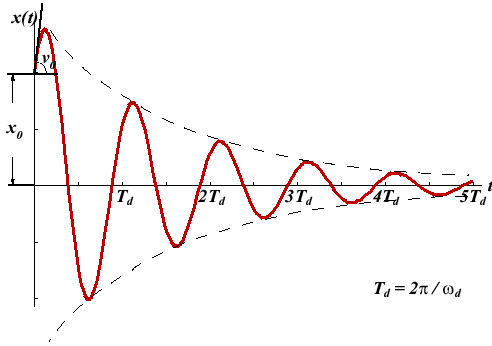
\includegraphics[width=0.70\textwidth]{img/SDOF_UnderDamped_Response.png}
    \caption{The displacement plot of an underdamped system}
    \label{fig:SDOF-underdamped-response-png}
\end{figure}

Note that the displacement amplitude decays exponentially (i.e. the natural
logarithm of the amplitude ratio for any two displacements separated in time
by a constant ratio is a constant):

\begin{eqarray}
    \frac{A_k}{A_{k+1}} &=
    \frac{A_0 e^{-\zeta \omega_n \left( k T_d \right)} \cos{ \left( \phi_0 \right) }}
         {A_0 e^{-\zeta \omega_n \left[ (k+1) T_d \right]} \cos{ \left( \phi_0 \right) }}\\
                        &=
    \frac{e^{-\zeta \omega_n \left( k T_d \right)}}
         {e^{-\zeta \omega_n \left[ (k+1) T_d \right]}}\\
                        &= e^{\zeta \omega_n T_d}\\
    \implies \ln{\left( \frac{A_k}{A_{k+1}} \right)} &=
    \zeta \omega_n T_d = \zeta \omega_n \frac{2 \pi}{\omega_d}
    = \frac{2 \pi \zeta}{\sqrt{1 - \zeta^2}}
\end{eqarray}

where $ T_d = \frac{1}{f_d} = \frac{2 \pi}{\omega_d} $ is the period of the
damped vibration.


\subsubsection{Time Solution of Unforced Critically-Damped Systems}

When $ c_v^2 - 4 m k = 0 $ (equivalent to $ \zeta = 1 $ or $ c_v = c_c $), the
characteristic equation has repeated real roots. The displacement solution for
this kind of system is:

\begin{eqarray}
    u(t) &= \left( c_1 + c_2 t \right) e^{-\omega_n t}\\
    \implies u(t) &= e^{-\omega_n t} \left[ u_0 + \left( v_0 + \omega_n u_0 \right) t \right]
\end{eqarray}

The critical damping factor $ c_c $ can be interpreted as the \textbf{minimum damping}
that results in non-periodic motion (i.e. simple decay).

\begin{figure}[ht]
    \centering
    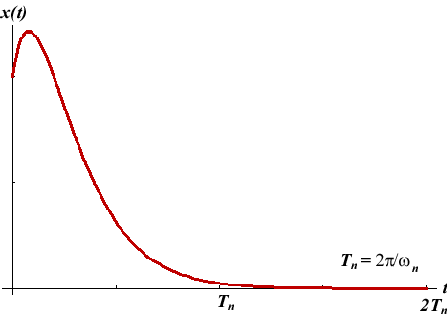
\includegraphics[width=0.70\textwidth]{img/SDOF_CriticalDamped_Response.png}
    \caption{The displacement plot of a critically-damped system with positive initial
displacement and velocity.}
    \label{fig:SDOF-critically-damped-response-png}
\end{figure}

The displacement decays to a negligible level after one natural period $ T_n $.
Note that if the initial velocity $ v_0 $ is negative while the initial displacement
$ u_0 $ is positive, there will exist one overshoot of the resting position in
the displacement plot.


\subsubsection{Time Solution of Unforced Overdamped SDOF Systems}

When $ c_v^2 - 4 m k > 0 $ (equivalent to $ \zeta > 1 $ or $ c_v > c_c $),
the characteristic equation has two distinct real roots. The displacement
solution for this kind of system is:

\begin{eqarray}
    u(t) &= c_1 e^{\left( -\zeta + \sqrt{\zeta^2 - 1} \right) \omega_n t}
          +  c_2 e^{\left( -\zeta - \sqrt{\zeta^2 - 1} \right) \omega_n t}\\
    \implies u(t) &=
    \frac{u_0 \omega_n \left( \zeta + \sqrt{\zeta^2 - 1} \right) + v_0}
    {2 \omega_n \sqrt{\zeta^2 - 1}} e^{\left( -\zeta + \sqrt{\zeta^2 - 1} \right) \omega_n t} +\\
                  &+
    \frac{-u_0 \omega_n \left( \zeta - \sqrt{\zeta^2 - 1} \right) - v_0}
    {2 \omega_n \sqrt{\zeta^2 - 1}} e^{\left( -\zeta - \sqrt{\zeta^2 - 1} \right) \omega_n t}
\end{eqarray}

\begin{figure}[ht]
    \centering
    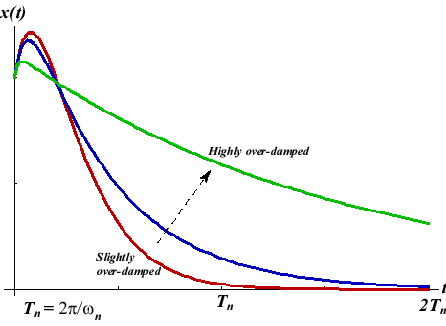
\includegraphics[width=0.70\textwidth]{img/SDOF_OverDamped_Response.png}
    \caption{The displaceent plot of an overdamped system response}
    \label{fig:SDOF-overdamped-response-png}
\end{figure}

The motion of an overdamped system is non-periodic, regardless of the inital conditions.
The larger the damping, the longer time to decay from an initial disturbance.

If the system is heavily damped, $ \zeta \gg 1 $, the displacement solution takes
the approximate form:

\begin{equation}
    u(t) \approx u_0 + \frac{v_0}{2 \zeta \omega_n}
    \left(1 - e^{-2 \zeta \omega_n t} \right)
\end{equation}


\subsection{SDOF Systems under Harmonic Excitaion}
\textit{https://www.efunda.com/formulae/vibrations/sdof\_harmo.cfm}

When a \textbf{SDOF} System is forced by $ f(t) $, the solution for the displacement
$ x(t) $ consists of two parts: the \textit{complimentary solution}, and the
\textit{particular solution}. The complimentary solution for the problem
is given by the \textbf{free vibration of an unforced SDOF System}.
The \textbf{particular solution} depends on the nature fo the forcing function.

When the forcing function is \textbf{harmonic} (i.e. it consits of at most
a \textbf{sine} and \textbf{cosine} at the same \textbf{frequency},
a quantity that can be expressed by the complex exponentional $ e^{i \omega t} $),
the method if \textbf{Undetermined Coefficients} can be used to find the particular
solution. Non-harmonic forcing functions are handled by other techniques.

Consider the SDOF system forced by the harmonic function $ f(t) $.

\begin{figure}[ht]
    \centering
    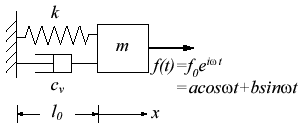
\includegraphics[width=0.70\textwidth]{img/SDOF_harmonic.png}
    \caption{SDOF System forced by the harmonic function $ f(t) $}
    \label{fig:SDOF-harmonic-response-png}
\end{figure}

The particular solution for this problem is found to be:

\begin{equation}
    u_p(t) = \frac{f_0}{ \left( k - m \omega^2 \right) + i c \omega} e^{i \omega t}
\end{equation}

The general solution is given by the sum of the complimentary and particular
solutions multiplied by two weighting constants $ c_1 $ and $ c_2 $,

\begin{equation}
    u(t) = c_1 u_c(t) + c_2 u_p(t)
\end{equation}

The values of $ c_1 $ and $ c_2 $ are found by matching $ u(t=0) $ to the
initial conditions.

\subsubsection{Undamped SDOF Systems under Harmonic Excitation}

For an undamped system ( $ c_v = 0 $ ) the total displacement solution is:

\begin{eqarray}
    u(t) &= d_1 \cos{\omega_n t} + d_2 \sin{\omega_n t} +
    \frac{f_0}{k - m \omega^2} e^{i \omega t}\\
    \implies u(t) &= \left( u_0 - \frac{f_0}{k - m \omega^2} \right) \cos{\omega_n t}\\
                  &+
    \left(\frac{v_0 - \frac{i \omega f_0}{k - m \omega^2}}{\omega_n} \right)
    \sin{\omega_n t}\\
                  &+ \frac{f_0}{k - m \omega^2} e^{i \omega t}
\end{eqarray}

If the forcing frequency is close to the natural frequency, $ \omega \approx \omega_n $,
the system will exhibit \textbf{resonance} (very large displacements) due to
near-zeros in the denominators of $ u(t) $.

When the forcing frequency is equal to the natural frequency, we cannot use the
$ u(t) $ given above as it would give divide-by-zero. Instead we must use
\textbf{L'H\^ospital's Rule} to derive a solution free of zeros in the denominators.

\begin{eqarray}
    u(t) &= u_0 \cos{\omega_n t} + \frac{v_0}{\omega_n} \sin{\omega_n t}\\
         &+ \lim_{\omega \rightarrow \omega_n} \left\{
             \frac{f_0}{k - m \omega^2} \left(
                 e^{i \omega t} - \cos{\omega_n t} - i \omega \sin{\omega_n t}
                 \right)
         \right\}\\
         &= u_0 \cos{\omega_n t} + \frac{v_0}{\omega_n} \sin{\omega_n t}
         - \frac{f_0 \omega_n}{2 k} \left(
             i t e^{i \omega)n t} - i \sin{\omega_n t}
             \right)
\end{eqarray}

To simplify $ u(t) $, let's assume that the driving force consists only of the
cosine function $ f(t) = f_0 \cos{\omega t} $.

\begin{figure}[ht]
    \centering
    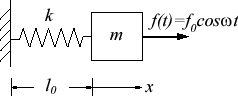
\includegraphics[width=0.35\textwidth]{img/SDOF_harmonic_undamped.png}
    \caption{SDOF System forced by the harmonic function $ f(t) = f_0 \cos{\omega t} $}
    \label{fig:SDOF-harmonic-undamped-response-png}
\end{figure}

The displacement solution reduces to:

\begin{eqarray}
    u(t) &= u_0 \cos{\omega_n t} + \frac{v_0}{\omega_n} \sin{\omega_n t}\\
         &+ \lim_{\omega \rightarrow \omega_n} \left\{
             \frac{f_0}{k - m \omega^2} \left(
                 \cos{\omega t} - \cos{\omega_n t}
                 \right)
         \right\}\\
         &= \underbrace{u_0 \cos{\omega_n t} + \frac{v_0}{\omega_n} \sin{\omega_n t}}_{
         free\ vibration\ (complementary)}
         + \underbrace{\frac{f_0 \omega_n t}{2 k}}_{\Scale[0.75]{
             \begin{matrix}
                 amplitude\\
                 linearly\\
                 increased
             \end{matrix}}}
         \sin{\omega_n t}
\end{eqarray}

This solution contains one term multiplied by $ t $. This term will cause the displacement
amplitude to increase linearly wit time as the forcing function pumps energy into
the system.

\begin{figure}[ht]
    \centering
    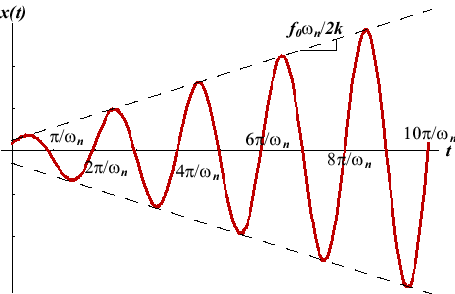
\includegraphics[width=0.70\textwidth]{img/SDOF_Undamped_Harmonic_Response.png}
    \caption{Resonance response of undamped SDOF with harmonic excitation}
    \label{fig:SDOF-undamped-harmonic-response-png}
\end{figure}

The maximum displacement of an undamped system forced at its resonant frequency will
increase unbounded according to the solution for $ u(t) $ above. However, real systems
will inject additional physics once displacements become large enough. These
additional physics (nonlinear plastic deformation, heat transfer, buckling etc.) will
serve to limit the maximum displacement exhibited by the system, and allow one to escape
the "sudden death" impression that such systems will immediately fail.


\subsubsection{Damped SDOF Systems under Harmonic Excitation}

\begin{equation}
    m \ddot{u} + c \dot{u} + k u = F_0 \cos{\left(\omega t \right)}
\end{equation}

then \textbf{steady state} solution is in the form:

\begin{equation}
    u_{s.s.} = u_0 \cos{\left(\omega t - \phi \right)}
\end{equation}

If we plug the \textbf{steady state} solution to the \textbf{equation of motion},
we get:

\begin{eqarray}
    u_o \left[ \left(k - m \omega^2\right) \cos{\omega t - \phi} -
    c \omega \sin{\left( \omega t - \phi \right)} \right]
    &= F_0 \cos{\left( \omega t \right)} \quad \vert \times \frac{1}{k}\\
        u_o \left[ \left(1 - \frac{\omega^2}{\omega_n^2} \right) \cos{\omega t - \phi} -
        2 \zeta \frac{\omega}{\omega_n} \sin{\left( \omega t - \phi \right)} \right]
    &= \frac{F_0}{k} \cos{\left( \omega t \right)}
\end{eqarray}

because:
\begin{equation}
    \frac{k}{m} = \omega_n
\end{equation}

\begin{equation}
    \zeta = \frac{c}{c_c}
\end{equation}

\begin{equation}
    c = 2 m \sqrt{\frac{k}{m}} = 2 m \omega_n
\end{equation}

\begin{equation}
    \frac{c}{k} = \frac{\zeta c_c}{k} = \frac{\zeta 2 m \omega_n}{k}
    = \frac{2 \zeta \omega_n^2}{omega_n^2} = \frac{2 \zeta}{\omega_n}
\end{equation}

after utilising the sine and cosine relations:

\begin{eqarray}
    \cos{\left( \omega t - \phi \right)} &=
    \cos{\omega t} \cos{\phi} + \sin{\omega t} \sin{\phi}\\
    \sin{\left( \omega t - \phi \right)} &=
    \sin{\omega t} \cos{\phi} + \cos{\omega t} \sin{\phi}
\end{eqarray}

we get a set of two equatons:
\begin{eqarray}
    u_o \left[ \left(1 - \frac{\omega^2}{\omega_n^2} \right) \cos{\phi} +
    2 \zeta \frac{\omega}{\omega_n} \sin{\phi} \right] \cos{\omega t}
    &= \frac{F_0}{k} \cos{\left( \omega t \right)}\\
    u_o \left[ \left(1 - \frac{\omega^2}{\omega_n^2} \right) \sin{\phi} -
    2 \zeta \frac{\omega}{\omega_n} \cos{\phi} \right] \sin{\omega t}
    &= 0\\
\end{eqarray}

and when solving just for amplitudes this reduces to a set of two algebraic equations
which is then solved for $ u_0 $ and $ \phi $:
\begin{eqarray}
    u_o \left[ \left(1 - \frac{\omega^2}{\omega_n^2} \right) \cos{\phi} +
    2 \zeta \frac{\omega}{\omega_n} \sin{\phi} \right]
    &= \frac{F_0}{k}\\
    u_o \left[ \left(1 - \frac{\omega^2}{\omega_n^2} \right) \sin{\phi} -
    2 \zeta \frac{\omega}{\omega_n} \cos{\phi} \right]
    &= 0\\
\end{eqarray}

The solution (\textbf{transfer function}) is finally:
\begin{eqarray}
    u_0 &= \frac{\frac{F_0}{k}}{
        \left[
            \left( 1 - \frac{\omega^2}{\omega_n^2} \right)^2 +
            \left( 2 \zeta \frac{\omega}{\omega_n} \right)^2
    \right]^{\frac{1}{2}}}\\
    \phi &= \tan^{-1} \left(
        \frac{2 \zeta \frac{\omega}{\omega_n}}{
    1 - \frac{\omega^2}{\omega_n^2}} \right)
\end{eqarray}

where:\\
$ u_0 $ is displacement amplitude\\
$ \frac{F_0}{k} $ is displacement from static simulation.

\begin{equation}
    H_0 = \frac{\frac{F_0}{k}}{
        \left[
            \left( 1 - \frac{\omega^2}{\omega_n^2} \right)^2 +
            \left( 2 \zeta \frac{\omega}{\omega_n} \right)^2
    \right]^{\frac{1}{2}}}
\end{equation}





\newpage
\section{Damping}

\subsection{Rayleigh Damping}
\textit{https://www.simscale.com/knowledge-base/rayleigh-damping-coefficients/}

Let \textbf{Rayleigh Damping} be defined as:

\begin{equation}
    c = \alpha k + \beta m
\end{equation}

where:\\
$ c $ is damping value [-],\\
$ \alpha $ is stiffness dependent damping coefficient,\\
$ \beta $ is inertia (mass) dependent damping coefficient,\\
$ m $ is mass and\\
$ k $ is stiffness.

Thus, substituting this relation to the equation of motion:

\begin{eqarray}
    m \ddot(u) + \left(\alpha k + \beta m \right) \dot{u} + k u &= f(t) & \space \vert \times \frac{1}{m}\\
    \ddot{u} + \left(\alpha \frac{k}{m} + \beta \frac{m}{m} \right) \dot{u} + \frac{k}{m} u
    &= \frac{f(t)}{m} & \space \vert \frac{k}{m} = \omega_n^2 \\
    \ddot{u} + \left(\alpha \omega_n^2 + \beta \right) \dot{u} + \omega_n^2 u &= \frac{f(t)}{m} & \space
\end{eqarray}

Damping Ratio:

\begin{eqarray}
    \zeta &= \frac{c}{2 m \omega_n}\\
    \zeta &= \frac{1}{2 m \omega_n} \left( \alpha k + \beta m \right)\\
    \zeta &= \frac{1}{2} \left( \alpha \omega_n + \frac{\beta}{\omega_n} \right)
\end{eqarray}

where:\\
$ \zeta $ is damping ratio,\\
$ c $ is damping value [-],\\
$ m $ is mass and\\
$ \omega_n $ is natural frequency [rad/s]

Substituting back:

\begin{equation}
    \ddot{u} + 2 \zeta \omega_n \dot{u} + \omega_n^2 k u = \frac{f(t)}{m}
\end{equation}


When \textbf{Damping is proportional to inertia}:

In this case, the stiffness coefficient $ \alpha = 0 $ and thus:

\begin{equation}
    \zeta = \frac{\beta}{2 \omega_n}
\end{equation}

For a given constant value of $ \beta $, it is seen that the damping is inversely
proportional to the natural frequency, as shown in the illustration:

\begin{figure}[ht]
    \centering
    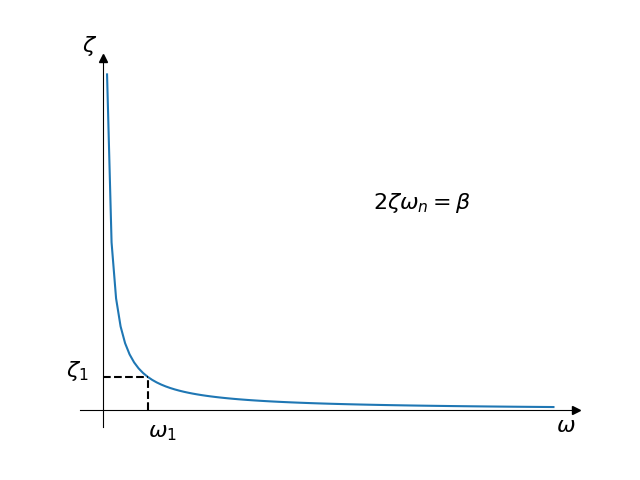
\includegraphics[width=0.90\textwidth]{img/inertia_dependent_damping.png}
    \caption{Schematic of damping proportional to inertia}
    \label{fig:inertia-dependent-damping-png}
\end{figure}

Moreover, if one computes $ \beta $ from the damping ration $ \zeta_1 $ at a given
natural frequency $ \omega_1 $, all the natural frequencies below it will be amplified
and the frequencies above it will be attenuated. The effect is more dramatic the farther
the frequencies are from the reference value.

When \textbf{Damping is proportional to stiffness}:

In this case, the mass coefficient $ \beta = 0 $ and thus:

\begin{equation}
    \zeta = \frac{1}{2} \alpha \omega_n
\end{equation}

It is seen that, contrary to the first case, here the damping id directly proportional
to the natural frequency:

\begin{figure}[ht]
    \centering
    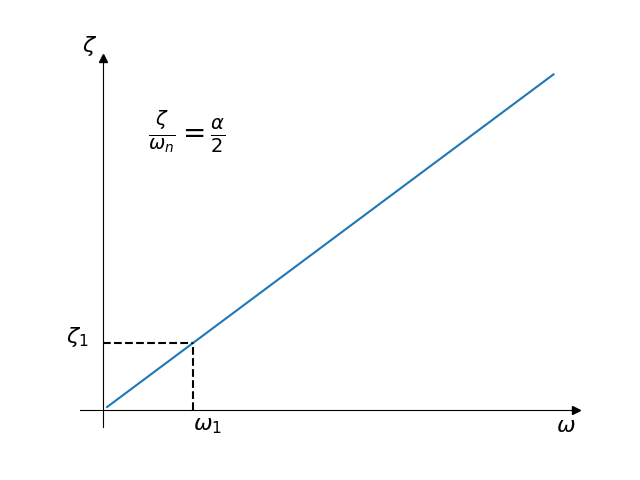
\includegraphics[width=0.90\textwidth]{img/stiffness_dependent_damping.png}
    \caption{Schematic of damping proportional to stiffness}
    \label{fig:stiffness-dependent-damping-png}
\end{figure}

If one computes $ \alpha $ from the damping ratio $ \zeta_1 $ at a natural
frequency $ \omega_1 $, then the natural frequencies below will be attenuated and
the frequencies above will be amplified.

\textbf{General Case}:

In the case of using the model with two parameters, the proportionality of damping
against frequency is convex:

\begin{figure}[ht]
    \centering
    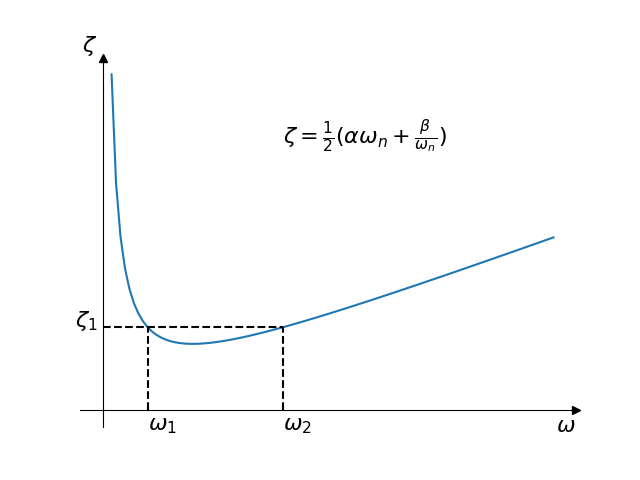
\includegraphics[width=0.90\textwidth]{img/general_rayleigh_damping.png}
    \caption{Schematic of full damping model}
    \label{fig:general-rayleigh-damping-png}
\end{figure}

In this case one needs two damping ratios and two natural frequencies to create
a pair of equations and solve for $ \alpha $ and $ \beta $. The model gives some
flexibility on where to place the natural frequencies, but in general, frequencies
too far away from the ones used in the computation will be amplified.

In the particular case of using equal damping ratios for the two frequencies,
it is important to note that the damping ratio \textbf{will not be constant inside the range}
defined by the sample points, but the inner frequencies will be attenuated. That is,
the inner frequencies will have a lower damping ratio.

\textbf{Computing the Rayleigh Damping Coefficients}

In the most common case, a transient response curve frim the system is obtained and
the damping ratio $ \zeta_1 $ is determined for the lowest natural frequency
$ \omega_1 $ by measuring the (logarithmic) attenuation of successive peaks.

\begin{figure}[ht]
    \centering
    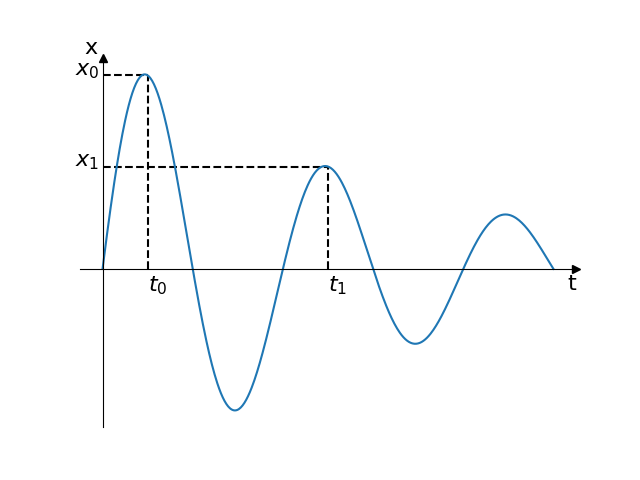
\includegraphics[width=0.90\textwidth]{img/Logarithmic_Decay_Damping_Ratio.png}
    \caption{Determination of the damping ration from the logarithmic decay}
    \label{fig:logarithmic-decay-damping-ratio-png}
\end{figure}

\begin{eqarray}
    \zeta &= \frac{\delta}{\sqrt{\delta^2 + (2 \pi)^2}}\\
    \delta &= \ln{\frac{x_0}{x_1}}\\
    f &= \frac{1}{T} = \frac{1}{t_1 - t_0}\\
    \omega &= 2 \pi f
\end{eqarray}

It is then most common to assume the case of damping proportional to the stiffness,
that is, $ \beta = 0 $, and the $ \alpha $ stiffness coefficient is computed from:

\begin{equation}
    \alpha = \frac{2 \zeta_1}{\omega_1} = \frac{\zeta+1}{\pi f_1}
\end{equation}

If the knowledge on the system indicates the case of damping decreasing with the
frequency, then one can assume the case of damping proportional to the inertia,
where $ \alpha = 0 $ and determine the mass coefficient $ \beta $:

\begin{equation}
    \beta = 2 \zeta_1 \omega_1 = 4 \pi \zeta_1 f_1
\end{equation}

If there is not such test data or knowledge of the system, or if one wishes to apply
an approximate damping ration over a range of frequencies, then we can use the
general case and build a system of two equations:

\begin{eqarray}
    \zeta_1 &= \frac{1}{2} \left( \alpha \omega_1 + \frac{\beta}{\omega_1} \right)\\
    \zeta_2 &= \frac{1}{2} \left( \alpha \omega_2 + \frac{\beta}{\omega_2} \right)
\end{eqarray}

Then solve for the unknown coefficients, keeping in mint the considerations given
above for the general case and the influence of the model on natural frequencies
inside and outside the range of interest. That is, perhaps one wants to achieve
a mean damping ratio over the range, then compensate the attenuation by modifying
the input damping rations, or by performing some least-squares approximation from
more than two frequency points.







\newpage
\section{Modal decomposition}

\subsection{Definition}

Let:

\begin{equation}
    \mathbf{M}\ddot{\mathbf{u}} + \mathbf{C}\dot{\mathbf{u}} +  \mathbf{K}\mathbf{u} = \mathbf{F}\left( t \right)
\end{equation}

be the \textbf{equation of motion}, then:\\
$ \mathbf{\Lambda} $ is a \textbf{spectral} matrix\\
$ \mathbf{\Psi} $ is a \textbf{mode shape} matrix,

such that:
\begin{equation}
    \mathbf{\Lambda} =
    \begin{bmatrix}
        \lambda_1^2 & \dots & 0\\
        \vdots & \ddots & \vdots \\
        0 & \dots & \lambda_n^2
    \end{bmatrix}
\end{equation}

where $ \lambda_n^2 $ is the n-th eigenvalue of the problem
$ (\mathbf{K}-\lambda^2\mathbf{M})\mathbf{X} = 0 $

and:
\begin{equation}
    \mathbf{\Psi} =
    \begin{bmatrix}
        \mathbf{\psi}_1 & \dots & \mathbf{\psi}_n
    \end{bmatrix}
\end{equation}

where $ \mathbf{\psi}_n = \{\psi_{n,1}, \dots, \psi_{n,m}\}^T $ is the eigenvector
of the n-th eigenvalue $ \lambda_n^2 $.

The \textbf{displacement} $ \mathbf{u} $ can be expressed as a linear combination
of eigenvectors such that:

\begin{eqarray}
    \mathbf{u}(t)
    &= \mathbf{\Psi} \mathbf{q}(t) \\
    &= \begin{bmatrix}
        \mathbf{\psi}_1 & \dots & \mathbf{\psi}_n
    \end{bmatrix} \mathbf{q}(t) \\
    &= \begin{bmatrix}
        \mathbf{\psi}_{1,1} & \dots & \mathbf{\psi}_{n,1} \\
        \vdots & \vdots & \vdots \\
        \mathbf{\psi}_{1,m} & \dots & \mathbf{\psi}_{n,m}
    \end{bmatrix}
    \begin{bmatrix}
        q_1(t) \\
        \vdots \\
        q_n(t)
    \end{bmatrix}
\end{eqarray}

where $ \mathbf{q}(t) $ is a vector of modal coefficients.

Then:

\begin{eqarray}
    \dot{\mathbf{u}}(t) &= \mathbf{\Psi} \dot{\mathbf{q}}(t) \\
    \ddot{\mathbf{u}}(t) &= \mathbf{\Psi} \ddot{\mathbf{q}}(t)
\end{eqarray}

First we substitute $ \mathbf{u} = \mathbf{\Psi}\mathbf{q} $ to the
\textbf{equation of motion}:

\begin{equation}
    \mathbf{M} \mathbf{\Psi} \ddot{q} +
    \mathbf{C} \mathbf{\Psi} \dot{q} +
    \mathbf{K}\mathbf{\Psi}\mathbf{q}
    = \mathbf{F}(t)
\end{equation}

By \textbf{premultiplying} with $ \mathbf{\Psi}^T $ we get:

\begin{equation}
    \mathbf{\Psi}^T \mathbf{M} \mathbf{\Psi} \ddot{\mathbf{q}} +
    \mathbf{\Psi}^T \mathbf{C} \mathbf{\Psi} \dot{\mathbf{q}} +
    \mathbf{\Psi}^T \mathbf{K} \mathbf{\Psi} \mathbf{q} =
    \mathbf{\Psi}\mathbf{F}(t) = \mathbf{Q}(t)
\end{equation}

where $ \mathbf{Q}(t) = \mathbf{\Psi} \mathbf{F}(t) $ is called a \textbf{modal load}.

\subsection{Orthonormalised Modal Base}

Then one can exploit the properties of \textbf{orthonormalised eigenvectors}, where:

\begin{equation}
    \mathbf{\psi}_r^T \mathbf{\psi}_s = 0 \Leftrightarrow r \neq s
\end{equation}

The \textbf{mass}, \textbf{damping} and \textbf{stiffness} matrices are therefore
reduced to:

\begin{eqarray}
    \mathbf{\Psi}^T \mathbf{M} \mathbf{\Psi}
    &= \begin{bmatrix}
        m_1 & \dots & 0 \\
        \vdots & \ddots & \vdots \\
        0 & \dots & m_n
    \end{bmatrix} \\
    \mathbf{\Psi}^T \mathbf{C} \mathbf{\Psi}
    &= \begin{bmatrix}
        c_1 & \dots & 0 \\
        \vdots & \ddots & \vdots \\
        0 & \dots & c_n
    \end{bmatrix} \\
    \mathbf{\Psi}^T \mathbf{K} \mathbf{\Psi}
    &= \begin{bmatrix}
        k_1 & \dots & 0 \\
        \vdots & \ddots & \vdots \\
        0 & \dots & k_n
    \end{bmatrix}
\end{eqarray}

where: \\
$ m_i $ is the \textbf{modal mass} of the i-th shape\\
$ c_i $ is the \textbf{modal damping} of the i-th shape\\
$ k_i $ is the \textbf{modal stiffness} of the i-th shape

\begin{bbox}[0.96]
    \textbf{Note}:

    When are the eigenvectors \textbf{orthonormalised} to \textbf{mass}, the above
    equations reduce to:

    \begin{eqarray}
        \mathbf{\Psi}^T \mathbf{M} \mathbf{\Psi}
        &= \begin{bmatrix}
            1.0 & \dots & 0 \\
            \vdots & \ddots & \vdots \\
            0 & \dots & 1.0
        \end{bmatrix} = \mathbf{I} \\
        \mathbf{\Psi}^T \mathbf{C} \mathbf{\Psi}
        &= \begin{bmatrix}
            c_1 & \dots & 0 \\
            \vdots & \ddots & \vdots \\
            0 & \dots & c_n
        \end{bmatrix} \\
        \mathbf{\Psi}^T \mathbf{K} \mathbf{\Psi}
        &= \begin{bmatrix}
            \lambda_1^2 & \dots & 0 \\
            \vdots & \ddots & \vdots \\
            0 & \dots & \lambda_n^2
        \end{bmatrix} = \mathbf{\Lambda}^2
    \end{eqarray}

    \textbf{Mass normalisation}:

    \begin{equation}
        \mathbf{\psi}_{i,mass} = \frac{\mathbf{\psi}_i}{\mathbf{\psi}_i^T \mathbf{m}_i \mathbf{\psi}_i}
    \end{equation}

    where:

    $ \mathbf{m}_i $ is the i-th row of the \textbf{mass} matrix $ \mathbf{M} $.

\end{bbox}


\subsection{MDOF to SDOF}

The MDOF \textbf{equation of motion} can be then rewritten as a set of \textbf{SDOF}
equations:

\begin{eqarray}
    \mathbf{\Psi}^T \mathbf{M} \mathbf{\Psi} \ddot{\mathbf{q}}(t) +
    \mathbf{\Psi}^T \mathbf{C} \mathbf{\Psi} \dot{\mathbf{q}}(t) +
    \mathbf{\Psi}^T \mathbf{K} \mathbf{\Psi} \mathbf{q}(t) &=
    \mathbf{\Psi}^T \mathbf{F}(t) \\
    \mathbf{M}_{\Psi} \ddot{\mathbf{q}}(t) +
    \mathbf{C}_{\Psi} \dot{\mathbf{q}}(t) +
    \mathbf{K}_{\Psi} \mathbf{q}(t) &= \mathbf{Q}(t)
\end{eqarray}

Written explicitely:

\begin{eqarray}
    \begin{bmatrix}
        m_1 & \dots & 0 \\
        \vdots & \ddots & \vdots \\
        0 & \dots & m_n
    \end{bmatrix}
    \begin{bmatrix}
        \ddot{q}_1(t) \\
        \vdots \\
        \ddot{q}_n(t)
    \end{bmatrix} &+ \\
    \begin{bmatrix}
        c_1 & \dots & 0 \\
        \vdots & \ddots & \vdots \\
        0 & \dots & c_n
    \end{bmatrix}
    \begin{bmatrix}
        \dot{q}_1(t) \\
        \vdots \\
        \dot{q}_n(t)
    \end{bmatrix} &+ \\
    \begin{bmatrix}
        k_1 & \dots & 0 \\
        \vdots & \ddots & \vdots \\
        0 & \dots & k_n
    \end{bmatrix}
    \begin{bmatrix}
        q_1(t) \\
        \vdots \\
        q_n(t)
    \end{bmatrix} &=
    \begin{bmatrix}
        Q_1(t) \\
        \vdots \\
        Q_n(t)
    \end{bmatrix}
\end{eqarray}

It is important to note that all modal matrices (mass, damping and stiffness) are
purely diagonal (with simple enough damping), so the \textbf{MDOF} problem reduces to a series
of \textbf{SDOF} problems:

\begin{eqarray}
    m_1 \ddot{q}_1(t) + c_1 \dot{q}_1(t) + k_1 q_1(t) &= Q_1(t) \\
    m_2 \ddot{q}_2(t) + c_2 \dot{q}_2(t) + k_2 q_2(t) &= Q_2(t) \\
    \vdots \\
    m_n \ddot{q}_n(t) + c_n \dot{q}_n(t) + k_n q_n(t) &= Q_n(t)
\end{eqarray}

which are solved separately and the results are \textbf{linearly} combined:

\begin{eqarray}
    \mathbf{u} = \sum_{i=1}^n \mathbf{\psi}_i q_i \\
    \mathbf{\dot{u}} = \sum_{i=1}^n \mathbf{\psi}_i \dot{q}_i \\
    \mathbf{\ddot{u}} = \sum_{i=1}^n \mathbf{\psi}_i \ddot{q}_i
\end{eqarray}

\begin{bbox}[0.96]
    \textbf{Note:} Above equation can be also written as:

    \begin{eqarray}
        \mathbf{u} = \sum_{i=1}^n \mathbf{\psi}_i q_{u,i} \\
        \mathbf{v} = \sum_{i=1}^n \mathbf{\psi}_i q_{v,i} \\
        \mathbf{a} = \sum_{i=1}^n \mathbf{\psi}_i q_{a,i}
    \end{eqarray}

    where:\\
    $ \mathbf{u} $ is displacement \\
    $ \mathbf{v} $ is velocity \\
    $ \mathbf{a} $ is acceleration

    and\\
    $ \mathbf{q}_{u} $ is modal displacement \\
    $ \mathbf{q}_v $ is modal velocity \\
    $ \mathbf{q}_a $ is modal acceleration

\end{bbox}


\subsection{Initial Conditions}

To get the initial modal conditions, one simply:

\begin{eqarray}
    \mathbf{q}_0 &= \mathbf{\Psi}^{-1} \mathbf{u}_0 \\
    \mathbf{\dot{q}}_0 &= \mathbf{\Psi}^{-1} \mathbf{\dot{u}}_0 \\
    \mathbf{\ddot{q}}_0 &= \mathbf{\Psi}^{-1} \mathbf{\ddot{u}}_0
\end{eqarray}

where:\\
$ \mathbf{\Psi}^{-1} $ is an inverse of eigenshape matrix $ \Leftrightarrow $ all eigenvalues
and eigenshapes are used.

\begin{bbox}[0.96]
    \textbf{Note}: This is not usually so. Normally one would use
    \textbf{reduced modal base}, where only the first \textbf{n} eigenmodes are used. Then
    $ \mathbf{\Psi}^{-1} $ is written as $ \mathbf{\Psi}^{+} $ and called the
    \textbf{pseudoinverse of mode shape matrix} defined (at least in \textbf{numpy}
    - \textit{numpy.linal.pinv()}) as:\\

    \smallskip
    The pseudo-inverse of a matrix $ \mathbf{A} $, denoted $ \mathbf{A}^{+} $,
    is defined as: “the matrix that ‘solves’ [the least-squares problem]
    $ \mathbf{A} \mathbf{x} = \mathbf{b} $ ,” i.e., if $ \overline{\mathbf{x}} $
    is said solution, then $ \mathbf{A}^{+} $ is that matrix such that
    $ \overline{\mathbf{x}} = \mathbf{A}^{+} \mathbf{b} $.\\

    \smallskip
    It can be shown that if $ \mathbf{Q}_1 \mathbf{\Sigma} \mathbf{Q}_2^T = \mathbf{A} $
    is the singular value decomposition of $ \mathbf{A} $, then
    $ \mathbf{A}^{+} = \mathbf{Q}_2 \mathbf{\Sigma}^{+} \mathbf{Q}_1^T $, where $ \mathbf{Q}_{1,2} $
    are orthogonal matrices, $ \mathbf{\Sigma} $  is a diagonal matrix consisting of
    $ \mathbf{A} $’s so-called singular values, (followed, typically, by zeros),
    and then $ \mathbf{\Sigma}^{+} $ is simply the diagonal matrix consisting
    of the reciprocals of $ \mathbf{A} $’s singular values (again, followed
    by zeros).
\end{bbox}




\chapter{Iterative Methods}

\section{second order ODE's}

Most of FEM problems are \textbf{second order Ordinary Differential Equations}, e.g:

\begin{eqarray}
    m \frac{u''(t)}{d^2 t} + c \frac{u'(t)}{dt} + k u(t) &= 0\\
    m \ddot{u} + c \dot{u} + k u &= 0\\
    m a + c v + ku &= 0
\end{eqarray}

while the iterative methods are for \textbf{first order ODE's} only.
A \textbf{substitution} technique is therefore used to transform the
\textbf{second order ODE's} to a set of \textbf{first order ODE's} and these are
then solved sequentialy.

First we begin with a \textbf{second order ODE} in the form of:

\begin{equation}
    a \frac{y''(x)}{d^2 x} + b \frac{y'(x)}{dx} + c y = d, \quad with \quad y(0) = y_0 \quad and \quad
    \frac{y'(0)}{dx} = y_1
\end{equation}

By stating:

\begin{equation}
    \frac{dy}{dx} = z
\end{equation}

and substituting back:

\begin{equation}
    a \frac{dz}{dx} + b z + c y = d
\end{equation}

now we can write the following set of equations:

\begin{eqarray}
    \begin{aligned}
        z &= \frac{dy}{dx}\\
        \frac{dz}{dx} &= \frac{d - c y - b z}{a}
    \end{aligned} &
    \quad \left\{
    \begin{aligned}
        y(0) &= y_0\\
        z(0) &= y_1
    \end{aligned} \right.
\end{eqarray}



\section{Explicit}

\subsection{Euler's method}
The \textbf{Euler's Method} is an iterative method to solve ODEs. This method's
huge plus is it is fast. The minus is it gradually diverges from the ideal solution.

The \textbf{Euler's Method} uses the following formula:

\begin{equation}
    y(t + h) = y(t) + h f(x,y)
\end{equation}

to construct the tangent at point $ x $ and obtain the value of $ y(x + h) $,
whose slope is:

\begin{equation}
    f(x,y) \quad or \quad \frac{dy}{dx}
\end{equation}

\begin{figure}[ht]
    \centering
    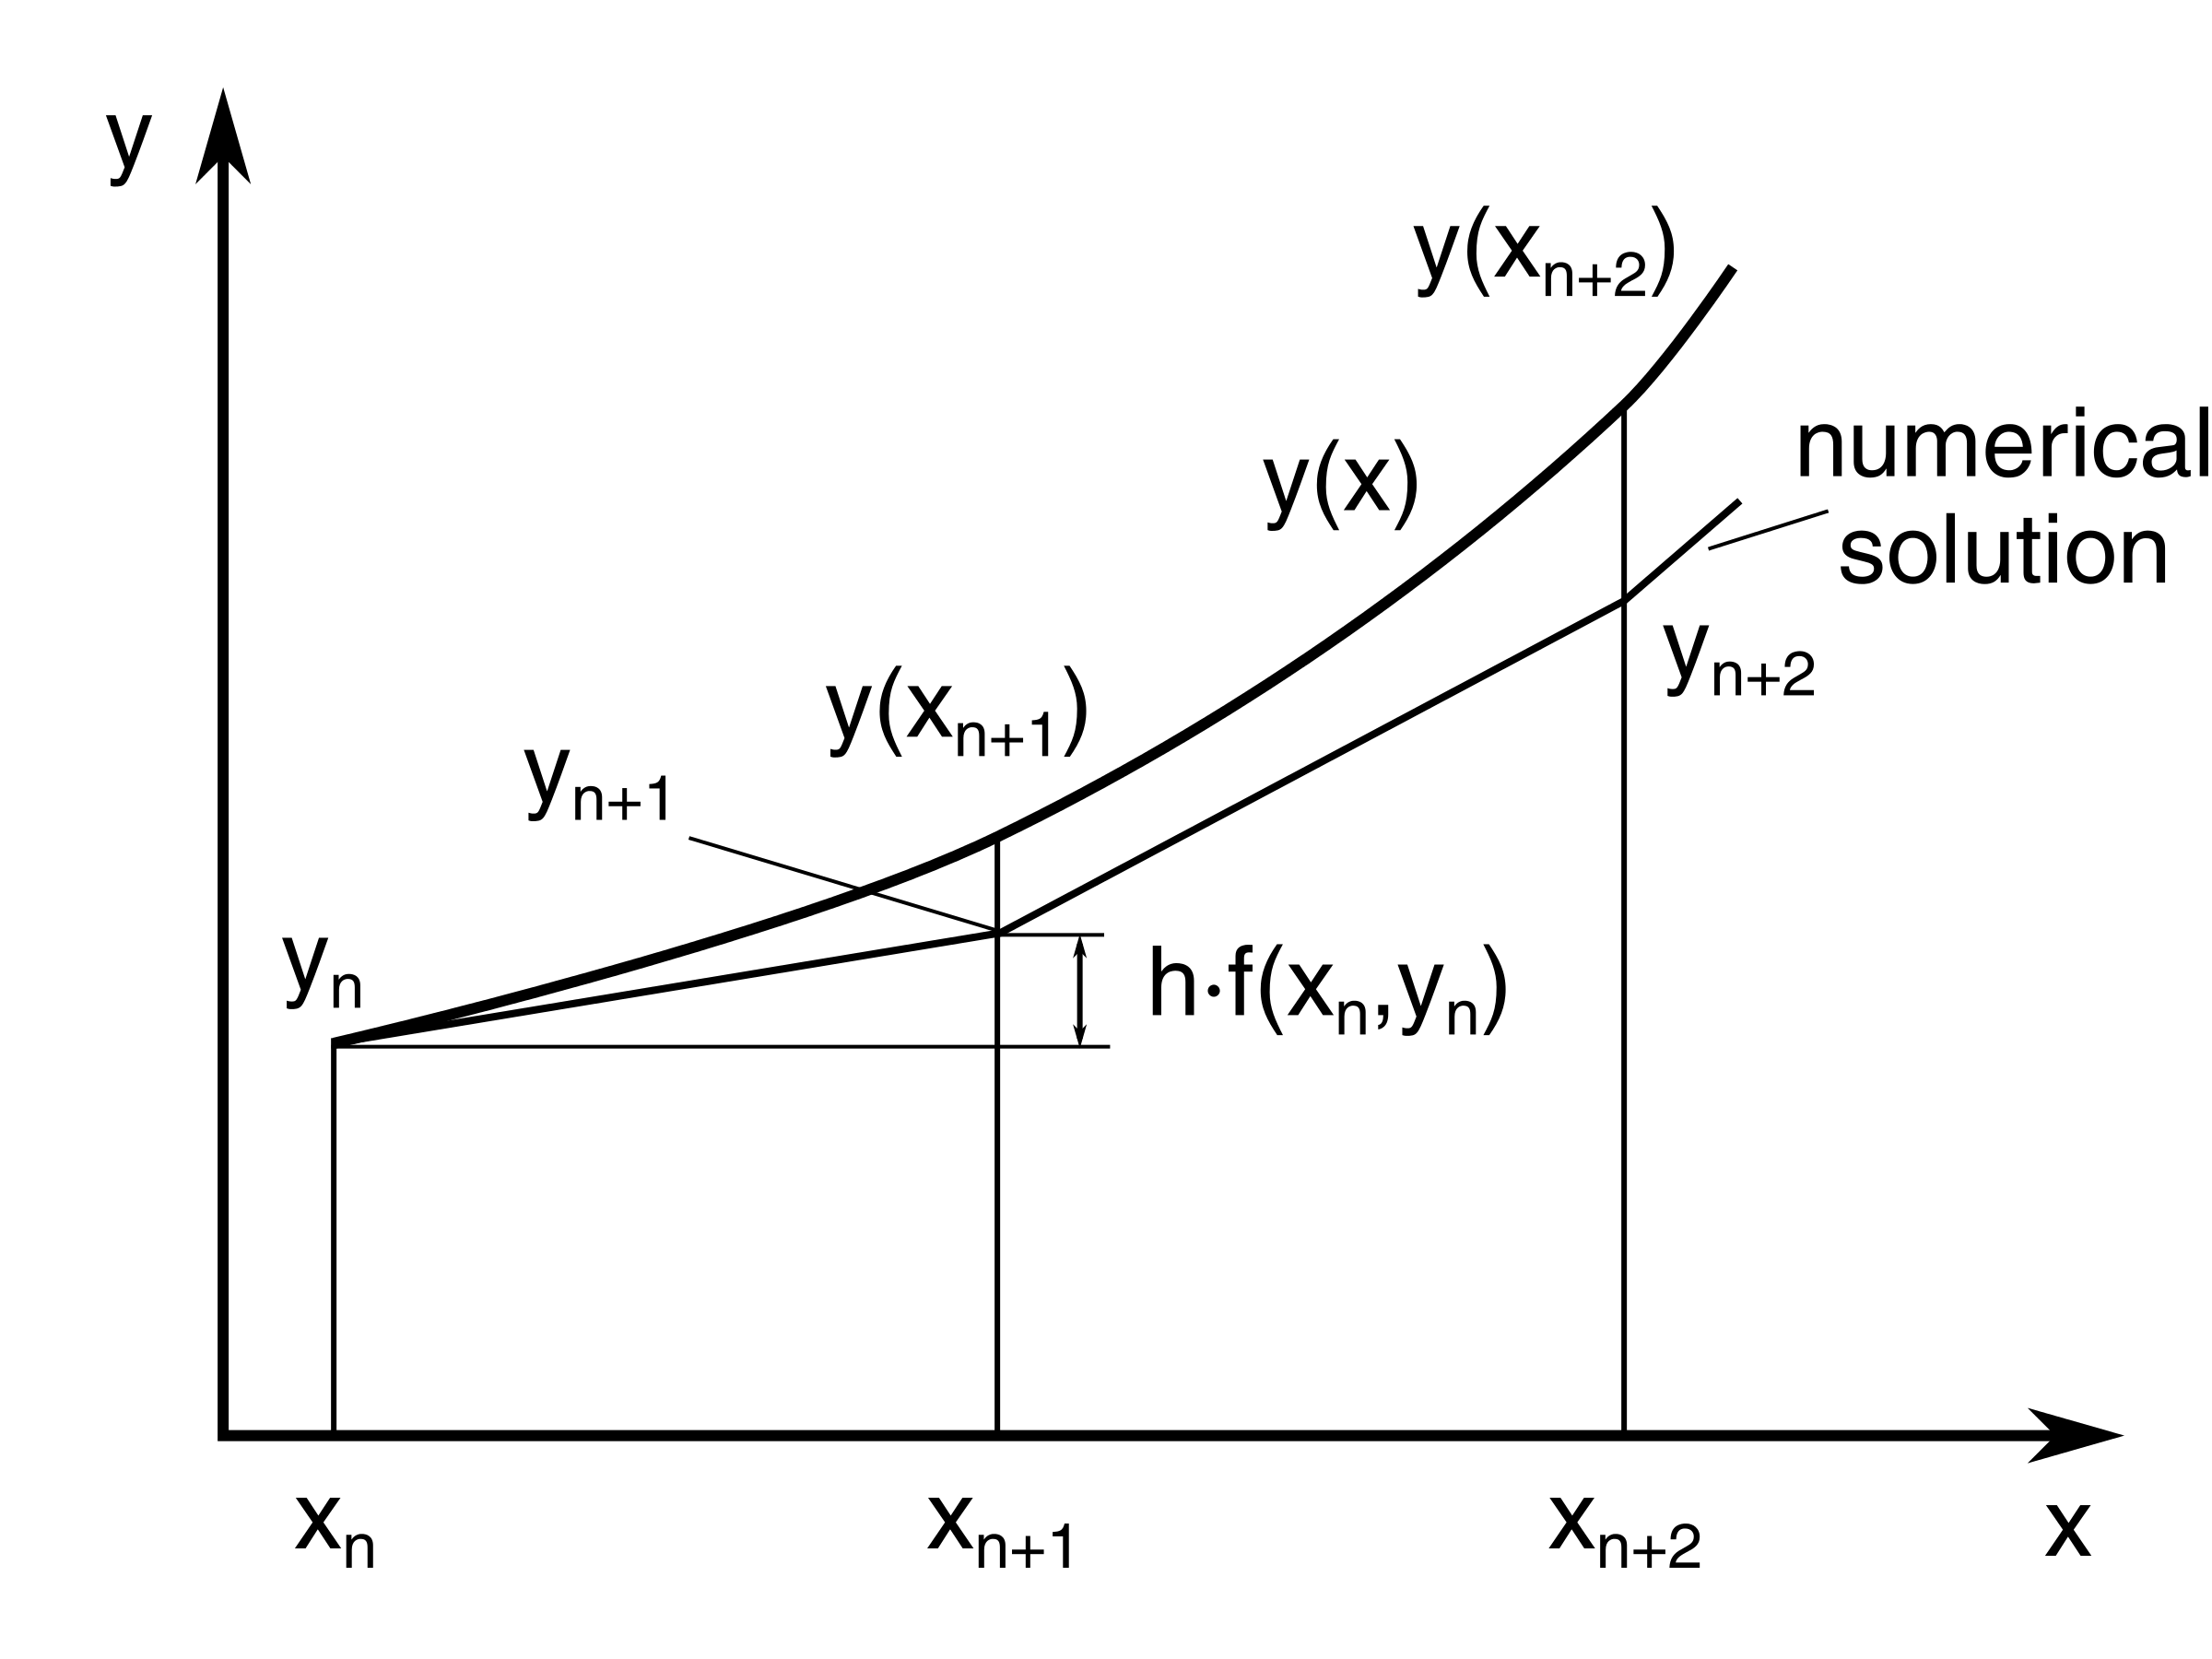
\includegraphics[width=0.90\textwidth]{img/Euler.png}
    \caption{Euler's method schematic}
    \label{fig:euler-png}
\end{figure}

In Euler's method, you can approximate the curve of the solution byt the tangent
in each interval (that is, by a sequence of shor line segments), at steps of $ h $.

\textit{In general}, if you use small step size, the accuracy of the approximation
increases.

\textbf{General Formula}

\begin{equation}
    y_{i+1} = y_i + h f(x_i,y_i)
\end{equation}

where:\\
$ y_{i+1} $ is the next estimated solution value,\\
$ y_i $ is the current value,\\
$ h $ is the interval between steps and\\
$ f(x_i,y_i) $ is the value of the derivative at the current $ (x_i,y_i) $ point.

\textbf{Pseudocode:}

\begin{itemize}
    \item define: $ f(x,y) $

    \item input: $ x_0 $, $ y_0 $

    \item input: $ h $, $ n $

    \item for $ j $ from $ 0 $ to $ (n-1) $ do
        \begin{itemize}
            \item $ y_{j+1} = y_j + hf(x_j, y_j) $
            \item $ x_{j+1} = x_j + h $
            \item Print $ x_{j+1} $ and $= y_{j+1} $
        \end{itemize}
    \item End.
\end{itemize}


\begin{bbox}[0.96]
\textbf{Note:}

If thinking about a problem in time domain:

\begin{itemize}
    \item define: $ f(t,x) $

    \item input: $ t_0 $, $ x_0 $

    \item input: $ dt $, $ n $

    \item for $ j $ from $ 0 $ to $ (n-1) $ do
        \begin{itemize}
            \item $ x_{j+1} = x_j + dt f(t_j, x_j) $
            \item $ t_{j+1} = t_j + dt $
            \item Print $ t_{j+1} $ and $= x_{j+1} $
        \end{itemize}
    \item end.
\end{itemize}

\end{bbox}


\newpage
\textbf{Python Code for vibration problem:}

\begin{python}
#!/usr/bin/python3
import numpy as np
import matplotlib.pyplot as plt


def iterate(h, y0, func, rhs):
    num_of_odes = y0.shape[0]
    y1 = np.zeros(num_of_odes, dtype = float)
    for i in range(num_of_odes-1):
        y1[i] = y0[i] + y0[i+1] * h
    y1[-1] = func(y1, rhs)
    return y1


def euler(t, y, func, rhs):
    N = t.shape[0]
    for j in range(N-1):
        dt = t[j+1] - t[j]
        y[j+1,:] = iterate(dt, y[j,:], func, rhs[j])
        # print(y[j+1,:])
    return y


def euler_vibration():
    m = 0.55  # tonnes
    c = 3.    # Ns/mm
    k = 1000. # N/mm

    freq = np.sqrt(k / m) / (2 * np.pi)

    # equation to solve
    # m * a + c * v + k * u = f
    # a = (f - c * v - k * u) / m
    acceleration = lambda u, f: (f - c * u[1] - k * u[0]) / m

    T = 2.0     # seconds
    dt = 0.0001 # timestep s
    u_0 = 0.    # mm of initial displacement
    v_0 = 0.    # mm/s of initial velocity

    # times at which to solve
    t = np.linspace(0, T, int(T/dt) + 1)

    # force vector
    F = 5000. # N of max impulse
    t0 = 0.1  # impulse start time
    t1 = 0.2  # impuls end time
    f = np.zeros(t.shape[0], dtype=float)
    # create a half sine impulse of force
    for i in range(t.shape[0]):
        if t[i] >= t0 and t[i] <= t1:
            f[i] = F * np.sin((t[i] - t0) / (t1 - t0) * np.pi)
        else:
            f[i] = 0.

    uva = np.zeros((t.shape[0],3), dtype=float)
    uva[0,0] = u_0
    uva[0,1] = v_0

    uva = euler(t, uva, acceleration, f)

    fig, axf = plt.subplots()
    fig.subplots_adjust(right=0.60)

    p1, = axf.plot(t, f, label='force', color='violet')
    axu = axf.twinx()
    p2, = axu.plot(t, uva[:,0], label='displacement', color='red')
    axv = axf.twinx()
    axv.spines.right.set_position(('axes', 1.20))
    p3, = axv.plot(t, uva[:,1], label='velocity', color='blue')
    axa = axf.twinx()
    axa.spines.right.set_position(('axes', 1.40))
    p4, = axa.plot(t, uva[:,2], label='acceleration', color='green')

    axf.set_xlabel('Time [s]')
    axf.set_ylabel('Force [N]')
    axu.set_ylabel('Displacement [mm]')
    axv.set_ylabel('Velocity [mm/s]')
    axa.set_ylabel('Acceleration [mm/s2]')

    axf.legend(handles=[p1, p2, p3, p4])

    plt.show()

if __name__ == '__main__':
    euler_vibration()

\end{python}

Which results to:
\begin{figure}[ht]
    \centering
    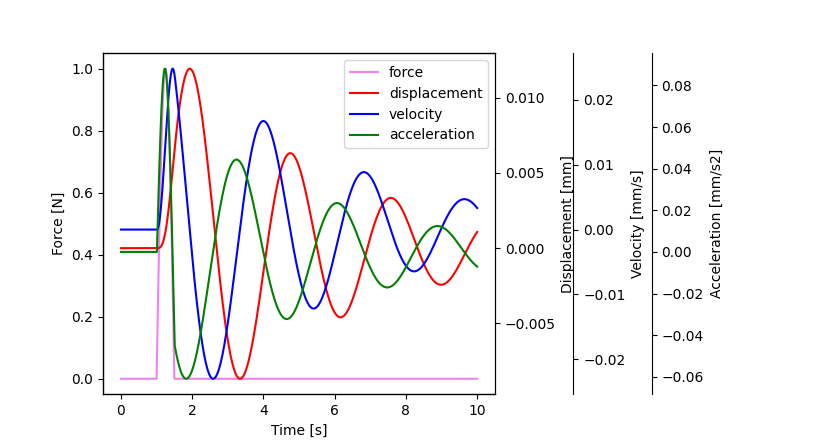
\includegraphics[width=0.90\textwidth]{img/euler_example.png}
    \caption{Euler's implementation for vibration problem example}
    \label{fig:euler-example-png}
\end{figure}


The \textbf{iterate()} function:
\begin{python}
def iterate(h, y0, func, rhs):
    num_of_odes = y0.shape[0]
    y1 = np.zeros(num_of_odes, dtype = float)
    for i in range(num_of_odes-1):
        y1[i] = y0[i] + y0[i+1] * h
    y1[-1] = func(y1, rhs)
    return y1

\end{python}

is written for general case of a set of ODEs. When considering the problem
of vibration (set of 2 ODEs):
\begin{python}
def iterate(h, u0, v0, a0, f, m , c, k):
    u1 = u0 + h * v0
    v1 = v0 + h * a0
    # m * a + c * v + k * u = f
    a1 = (f - c * v1 - k * u1) / m
    return np.array([u1, v1, a1], dtype=float)
\end{python}

which is the iteration of a set of \textbf{first order ODEs}:
\begin{eqarray}
    v &= \dot{u}\\
    \dot{v} &= \frac{f - c * v - k * u}{m}
\end{eqarray}

\newpage
\subsection{Runge-Kutta 4th order method}

\textbf{Runge-Kutta 4th order method} is another explicit method for solving
\textbf{first order ODEs}. The basic equation is:

\begin{equation}
    \frac{dy}{dx} = f(x,y) \quad , y(0) = y_0
\end{equation}

The formula for the next value $ y_{i+1} $ after a step size equal to $h $ is given by:

\begin{eqarray}
    k_1 &= h f(x_i, y_i)\\
    k_2 &= h f(x_i + \frac{h}{2}, y_i + \frac{k_1}{2})\\
    k_3 &= h f(x_i + \frac{h}{2}, y_i + \frac{k_2}{2})\\
    k_4 &= h f(x_i + h, y_i + k_3)\\
    y_{i+1} &= y_i + \frac{k_1}{6} + \frac{k_2}{3} + \frac{k_3}{3} + \frac{k_4}{6} + O(h^5)
\end{eqarray}

The formula basically computes next value $ y_{i+1} $ using current $ y_i $ plus
\textbf{weighted average of four increments}:

\begin{itemize}
    \item $ k_1 $ is the increment based on the slope at the beginning of the
    interval, using $ y $

    \item $ k_2 $ is the increment based on the slope at the midpoint of the interval,
        using $ y + h k_1 / 2 $

    \item $ k_3 $ is the increment based on the slope at the midpoint,
        using $ y + h k_2 / 2 $

    \item $ k_4 $ is the increment based on the slope at the end of the interval,
        using $ y + h k_3 / 2 $

\end{itemize}

The method is a fourth order method, meaning that the local truncation error is
on the order of $ O(h^5) $, while the total accumulated error is of order $ O(h^4) $.

\begin{figure}[ht]
    \centering
    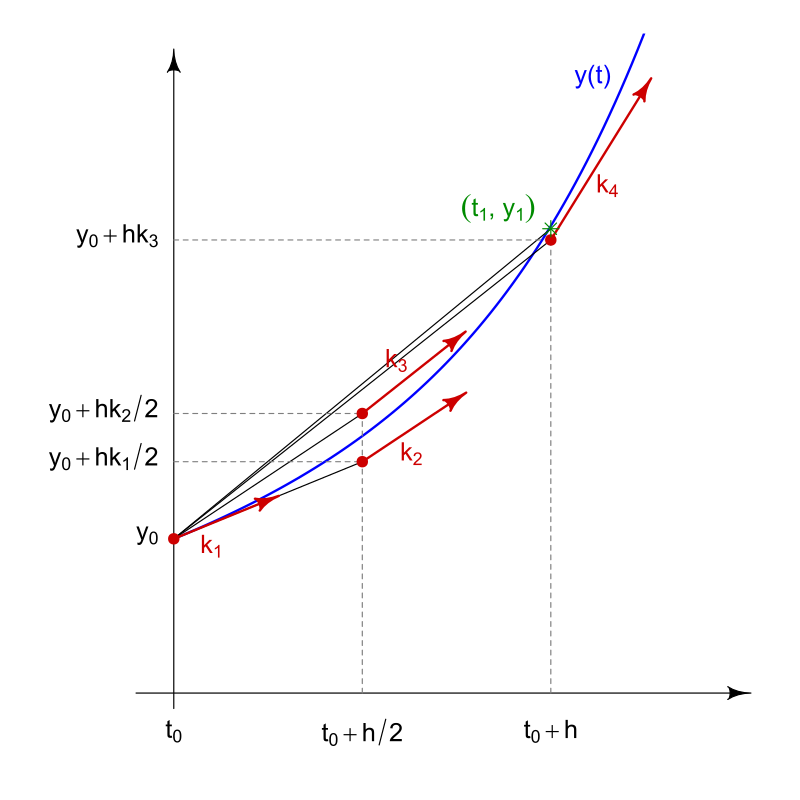
\includegraphics[width=0.80\textwidth]{img/Runge-Kutta_slopes.png}
    \caption{4th Order Runge-Kutta's method schematic}
    \label{fig:rk4-schema-png}
\end{figure}

\newpage
\begin{bbox}[0.96]
\textbf{Note:}

The formula for the next value $ y_{i+1} $ can be also written as:

\begin{eqarray}
    k_1 &= y_i\\
    k_2 &= y_i + \frac{h}{2} \frac{d k_1}{dx}\\
    k_3 &= y_i + \frac{h}{2} \frac{d k_2}{dx}\\
    k_4 &= y_i + h \frac{k_3}{dx}\\
    y_{i+1} &= y_i + \frac{h}{6} (\frac{d k_1}{dx} + 2 \frac{d k_2}{dx}
                              + 2 \frac{d k_3}{dx} + \frac{d k_4}{dx}) + O(h^5)
\end{eqarray}
\end{bbox}

\begin{bbox}[0.96]
This notation is more convenient to use when solving sets of ODEs for vibration
problem, because it translates to:

\begin{eqarray}
    u_1 &= u_0\\
    v_1 &= v_0\\
    a_1 &= (f - c v_0 - k u_0) / m\\
    u_2 &= u_0 + \frac{h}{2} v_1\\
    v_2 &= v_0 + \frac{h}{2} a_1\\
    a_2 &= (f - c v_1 - k u_1) / m\\
    u_3 &= u_0 + \frac{h}{2} v_2\\
    v_3 &= v_0 + \frac{h}{2} a_2\\
    a_3 &= (f - c v_2 - k u_2) / m\\
    u_4 &= u_0 + h v_3\\
    v_4 &= v_0 + h a_3\\
    a_4 &= (f - c v_3 - k u_3) / m\\
    u_{i+1} &= u_0 + \frac{h}{6} \left( v_1 + 2 v_2 + 2 v_3 + v_4 \right) \\
    v_{i+1} &= v_0 + \frac{h}{6} \left( a_1 + 2 a_2 + 2 a_3 + a_4 \right) \\
    a_{i+1} &= (f - c v_{i+1} - k u_{i+1}) / m\\
\end{eqarray}

where each of the \textbf{ODEs} are solved sequentially from the values
already known.

\end{bbox}

\newpage
\textbf{Python implementation for vibration problem:}

\begin{python}
#!/usr/bin/python3
import numpy as np
import matplotlib.pyplot as plt


def iterate(h, y0, y, func, rhs):
    num_of_odes = y0.shape[0]
    y1 = np.zeros(num_of_odes, dtype = float)
    for i in range(num_of_odes-1):
        y1[i] = y0[i] + y[i+1] * h
    y1[-1] = func(y1, rhs)
    return y1


def runge_kutta_4(t, y, func, rhs):
    N = t.shape[0]
    for j in range(N-1):
        dt = t[j+1] - t[j]
        y1 = iterate(0., y[j,:], y[j,:], func, rhs[j])
        y2 = iterate(dt/2, y[j,:], y1, func, 0.5 * (rhs[j+1] + rhs[j]))
        y3 = iterate(dt/2, y[j,:], y2, func, 0.5 * (rhs[j+1] + rhs[j]))
        y4 = iterate(dt, y[j,:], y3, func, rhs[j+1])

        # next step solution
        for i in range(y.shape[1]-1):
            y[j+1,i] = y[j,i] + dt/6 * (y1[i+1] + 2 * y2[i+1] + 2 * y3[i+1] + y4[i+1])
        y[j+1,-1] = func(y[j+1,:], rhs[j+1])
    return y


def rk4_vibration():
    m = 10.   # tonnes
    c = 5.    # Ns/mm
    k = 50.   # N/mm

    freq = np.sqrt(k / m) / (2 * np.pi)
    print(f'f = {freq}')

    # equation to solve
    # m * a + c * v + k * u = f
    # a = (f - c * v - k * u) / m
    acceleration = lambda u, f: (f - c * u[1] - k * u[0]) / m

    T = 10.     # seconds
    dt = 0.01   # timestep s
    u_0 = 0.    # mm of initial displacement
    v_0 = 0.    # mm/s of initial velocity

    # times at which to solve
    t = np.linspace(0, T, int(T/dt) + 1)

    # force vector
    F = 1.    # N of max impulse
    t0 = 1.   # impulse start time
    t1 = 1.5  # impuls end time
    f = np.zeros(t.shape[0], dtype=float)
    # create a half sine impulse of force
    for i in range(t.shape[0]):
        if t[i] >= t0 and t[i] <= t1:
            f[i] = F * np.sin((t[i] - t0) / (t1 - t0) * np.pi)
        else:
            f[i] = 0.

    uva = np.zeros((t.shape[0],3), dtype=float)
    uva[0,0] = u_0
    uva[0,1] = v_0

    uva = runge_kutta_4(t, uva, acceleration, f)

    fig, axf = plt.subplots()
    fig.subplots_adjust(right=0.60)

    p1, = axf.plot(t, f, label='force', color='violet')
    axu = axf.twinx()
    p2, = axu.plot(t, uva[:,0], label='displacement', color='red')
    axv = axf.twinx()
    axv.spines.right.set_position(('axes', 1.20))
    p3, = axv.plot(t, uva[:,1], label='velocity', color='blue')
    axa = axf.twinx()
    axa.spines.right.set_position(('axes', 1.40))
    p4, = axa.plot(t, uva[:,2], label='acceleration', color='green')

    axf.set_xlabel('Time [s]')
    axf.set_ylabel('Force [N]')
    axu.set_ylabel('Displacement [mm]')
    axv.set_ylabel('Velocity [mm/s]')
    axa.set_ylabel('Acceleration [mm/s2]')

    axf.legend(handles=[p1, p2, p3, p4])

    plt.show()

if __name__ == '__main__':
    rk4_vibration()

\end{python}

Which results to:
\begin{figure}[ht]
    \centering
    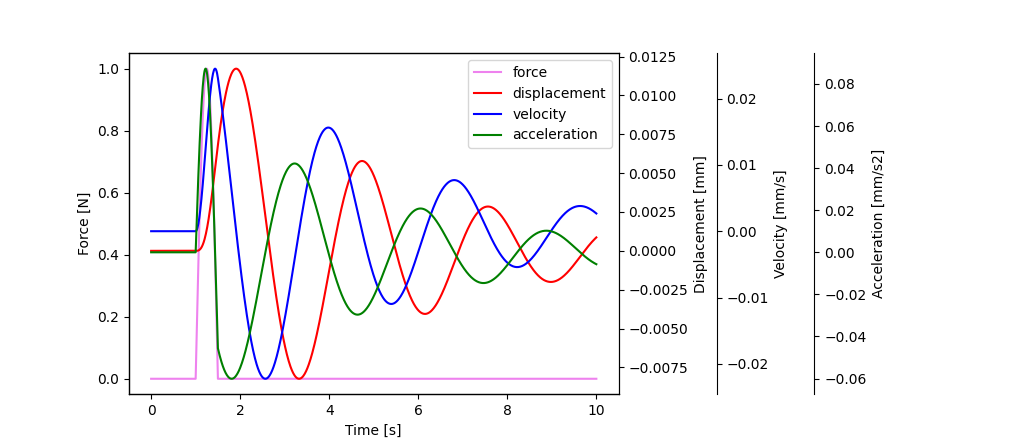
\includegraphics[width=0.90\textwidth]{img/rk4_example.png}
    \caption{4th order Runge-Kutta's implementation for vibration problem example}
    \label{fig:rk4-example-png}
\end{figure}



\newpage
\chapter{Element Atlas}

\section{Matrices}

\textbf{The inversion formula for 3x3 matrix:}

\begin{eqarray}
    \mathbf{A} &=
    \begin{bmatrix}
        a_{11} & a_{12} & a_{13}\\
        a_{21} & a_{22} & a_{23}\\
        a_{31} & a_{32} & a_{33}
    \end{bmatrix}\\
    \mathbf{A}^{-1} &= \frac{1}{\vert \mathbf{A} \vert}
    \begin{bmatrix}
        A_{11} & A_{12} & A_{13}\\
        A_{21} & A_{22} & A_{23}\\
        A_{31} & A_{32} & A_{33}
    \end{bmatrix}\\
\end{eqarray}

where:
\begin{eqarray}
    A_{11} &= a_{22} a_{33} - a_{23} a_{32}\\
    A_{22} &= a_{33} a_{11} - a_{31} a_{13}\\
    A_{33} &= a_{11} a_{22} - a_{12} a_{21}\\
    A_{12} &= a_{23} a_{31} - a_{21} a_{33}\\
    A_{23} &= a_{31} a_{12} - a_{32} a_{11}\\
    A_{31} &= a_{12} a_{23} - a_{13} a_{22}\\
    A_{21} &= a_{32} a_{13} - a_{12} a_{33}\\
    A_{32} &= a_{13} a_{21} - a_{23} a_{11}\\
    A_{13} &= a_{21} a_{22} - a_{31} a_{22}\\
    \vert A_{13} \vert &= a_{11} A_{11} + a_{12} A_{21} + a_{13} A_{31}
\end{eqarray}


\section{Numerical Integration}

\begin{bbox}
    \textbf{Note:}

    \textbf{Quadrature} is another term for \textbf{Numerical Integration}.
\end{bbox}


\subsection{Newton-Cotes quadrature}
In the most obvious procedure, points at which the function is to be formed are
determined \textit{a priori} - usually at equal intervals - and a polynomial
passed through the values of the function at these points and exactly integrated.

As $ n $ values define a polynomial of degree $ n - 1 $, the errors will be
of the order $ O(h^n) $ where $ h $ is the element size. This leads to the
well-known \textbf{Newton-Cotes} \'quadrature formulae\'. The integrals can be
written as:

\begin{equation}
    I = \int_{-1}^{1} f(\xi) d\xi = \sum_1^n H_i f(\xi_i)
\end{equation}

for the range of integration between $ -1 $ and $ +1 $. For example, if $ n = 2 $,
we have the well-known trapezoidal rule:

\begin{equation}
    I = f(-1) + f(1)
\end{equation}

for $ n = 3 $, the well-known \textbf{Simpson} one-third rule:

\begin{equation}
    I = \frac{1}{3} \left[ f(-1) + 4f(0) + f(1) \right]
\end{equation}

and for $ n = 4 $:

\begin{equation}
    I = \frac{1}{4} \left[f(-1) + 3f(-\frac{1}{3}) + 3f(\frac{1}{3}) + f(1) \right]
\end{equation}


\subsection{Gauss quadrature}

If in place of specifying the position of sampling points \textit{a priori} we
allow these to be located at points to be determined so as to aim for best
accuracy, then for a given number of sampling points increased accuracy can be
obtained. Indeed, if we again consider:

\begin{equation}
    I = \int_{-1}^{1} f(\xi) d\xi = \sum_1^n H_i f(\xi_i)
\end{equation}

and again assume a polynomial expression, it is easy to see that for $ n $ sampling
points we have $ 2n $ unknowns ($H_i$ and $\xi_i$) and hence a polynomial of degree
$ 2n-1 $ could be constructed and exactly integrated. The error is thus of order
$ O(h^{2n}) $.

The simultaneous equations involved are difficult to solve, but some mathematical
manipulation will show that the solution can be obtained explicitely in terms
of \textbf{Legendre polynomials}. Thus this particular process is frequently known
as \textbf{Gauss-Legendre} quadrature.

For purposes of finite elements analysis complex calculations are involved in
determining the values of $ f $, the function to be integratet. Thus the
Gauss-type processes, requiring the least number of such evaluations, are ideally
suited and are mostly used exvlusively.

Other expresssions for integration of functions of the type

\begin{equation}\label{leggaus}
    I = \int_{-1}^{1} w(\xi) f(\xi) d\xi = \sum_{1}^{n} H_i f(\xi_i)
\end{equation}

can be derived for prescribed forms of $ w(\xi) $, again integrating up to a certain
order of accuracy a polynomial expansion of $ f(\xi) $.


\subsection{Linear and Quadrilateral Elements}

\subsubsection{For 1D:}

\begin{equation}
    I = \int_{-1}^{1} f(\xi) d\xi = \sum_1^n H_i f(\xi_i)
\end{equation}


\subsubsection{For 2D:}

The most obvious way of obtaining the integral:

\begin{equation}
    I = \int_{-1}^{1} \int_{-1}^{1} f(\xi, \eta) d\xi d\eta
\end{equation}

Is to first evaluate the inner integral keeping $ \eta $ constant, i.e.:

\begin{equation}
    \int_{-1}^{1}f(\xi, \eta) d\xi = \sum_{j=1}^n H_j f(\xi_i, \eta) = \psi(\eta)
\end{equation}

Evaluating the outer integral in a similar manner, we have:

\begin{eqarray}
    I = \int_{-1}^{1} \psi(\eta) d\eta
    &= \sum_{i=1}^n H_i \psi(\eta_i)\\
    &= \sum_{i=1}^n H_i \sum_{j=1}^n H_j f(\xi_i,\eta_i)\\
    &= \sum_{i=1}^n \sum_{j=1}^n H_i H_j f(\xi_j,\eta_i)
\end{eqarray}

\subsubsection{For 3D:}
For a 3D element we have similarly:

\begin{eqarray}
    I &= \int_{-1}^{1} \int_{-1}^{1} \int_{-1}^{1} f(\xi, \eta, \mu) d\xi d\eta d\mu\\
    &= \sum_{i=1}^n \sum_{j=1}^n \sum_{k=1}^n H_i H_j f(\xi_i,\eta_j,\mu_k)
\end{eqarray}

In the above, the number of integrating points in each direction was assumed to be
the same. Clearly this is not necessary and on occasion it may be an advantage to
use different numbers in each direction of integration.

\begin{figure}[ht]
    \centering
    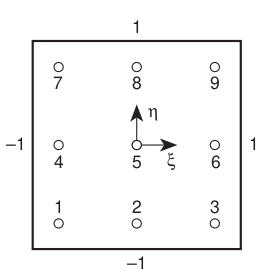
\includegraphics[width=0.25\textwidth]{img/quad_interpolation_3.png}
    \caption{Integration points for $ n = 3 $ in a square region. Exact for a
    polynomial of fifth order in each direction}
    \label{fig:quad-interpolation-3-png}
\end{figure}

\begin{table}
    \centering
    \renewcommand{\arraystretch}{1.25}
    \begin{tabular}{||c c c||}
        \hline
        \hline
        integration point & polynomial order & weight\\
        \hline
        \hline
        0 & n = 1 & 2.0\\
        \hline
        \begin{tabular}{c}
            $ -1/\sqrt{3} $ \\
            $ 1/\sqrt{3} $
        \end{tabular} & n = 2 &
        \begin{tabular}{c}
            1.0 \\
            1.0
        \end{tabular} \\
        \hline
        \begin{tabular}{c}
            $ -\sqrt{0.6} $ \\
            $ 0.0 $ \\
            $ \sqrt{0.6} $
        \end{tabular} & n = 3 &
        \begin{tabular}{c}
            $ 5/9 $ \\
            $ 8/9 $ \\
            $ 5/9 $
        \end{tabular} \\
        \hline
        \begin{tabular}{c}
            -0.861 136 311 594 953 \\
            -0.339 981 043 584 856 \\
             0.339 981 043 584 856 \\
             0.861 136 311 594 953 \\
        \end{tabular} & n = 4 &
        \begin{tabular}{c}
            0.347 854 845 137 454 \\
            0.652 145 154 862 546 \\
            0.652 145 154 862 546 \\
            0.347 854 845 137 454 \\
        \end{tabular} \\
        \hline
        \begin{tabular}{c}
            -0.906 179 845 938 664 \\
            -0.538 469 310 105 683 \\
             0.000 000 000 000 000 \\
             0.538 469 310 105 683 \\
             0.906 179 845 938 664 \\
        \end{tabular} & n = 5 &
        \begin{tabular}{c}
            0.236 926 885 056 189 \\
            0.478 628 670 499 366 \\
            0.568 888 888 888 889 \\
            0.478 628 670 499 366 \\
            0.236 926 885 056 189 \\
        \end{tabular} \\
        \hline
        \begin{tabular}{c}
            -0.932 469 514 203 152 \\
            -0.661 209 386 466 265 \\
            -0.238 619 186 083 197 \\
             0.238 619 186 083 197 \\
             0.661 209 386 466 265 \\
             0.932 469 514 203 152 \\
        \end{tabular} & n = 6 &
        \begin{tabular}{c}
            0.171 324 492 379 170 \\
            0.360 761 573 048 139 \\
            0.467 913 934 572 691 \\
            0.467 913 934 572 691 \\
            0.360 761 573 048 139 \\
            0.171 324 492 379 170 \\
        \end{tabular} \\
        \hline
        \begin{tabular}{c}
            -0.949 107 912 342 759 \\
            -0.741 531 185 599 394 \\
            -0.405 845 151 377 397 \\
             0.000 000 000 000 000 \\
             0.405 845 151 377 397 \\
             0.741 531 185 599 394 \\
             0.949 107 912 342 759 \\
        \end{tabular} & n = 7 &
        \begin{tabular}{c}
            0.129 484 966 168 870 \\
            0.279 705 391 489 277 \\
            0.381 830 050 505 119 \\
            0.471 959 183 673 469 \\
            0.381 830 050 505 119 \\
            0.279 705 391 489 277 \\
            0.129 484 966 168 870 \\
        \end{tabular} \\
        \hline
        \hline
    \end{tabular}
    \caption{Gauss-Legendre Integration Points and Weights}
\end{table}

\begin{bbox}
    To get the \textbf{Gauss-Legendre} points and weights in python use:

    \begin{python}
import numpy as np

# number of integration points
N = 3

points, weights = np.polynomial.legendre.leggauss(N)
    \end{python}
\end{bbox}


\newpage
\subsection{Triangular and Tetrahedral elements:}

\subsubsection{2D}
For a triangle, in terms of the \textbf{area coordinates} the integrals are of the
form:

\begin{equation}
    I = \int_{0}^{1} \int_{0}^{1-\xi} f(\xi, \eta, \mu) d\eta d\xi, \quad
    \mu = 1 - \xi - \eta
\end{equation}

Once again we could use $ n $ Gauss points and arrive at a summation expression of
the type used in the previous section. However, the limits of integration now
involve the variable itself and it is convenient to use alternative sampling points
for the second integration by use of a special Gauss expression for integrals of
the type given by equation \eqref{leggaus} in which $ w $ is a linear function.
These have been devised by \textit{Radau} and used successfully in finite element context.
It is, however, much more desirable (and aesthetically pleasing) to use special
formulae in which no bias is given to any of the natural coordinates ($\xi, \eta, \mu$).
Such formulae were first derived by \textit{Hammer et al.} and \textit{Felippa}
and a series of necessary sampling points and weights.

\newpage
\begin{table}[h!]
    \centering
    \renewcommand{\arraystretch}{1.25}
    % \small
    % \scriptsize
    \scalebox{0.80}{
    \begin{tabular}{||c c c c c c||}
        \hline
        \hline
        Order & Figure & Error & Points &
        \begin{tabular}{c} Triangular\\Coordinates\end{tabular} & Weights\\
        \hline
            Linear &
            \begin{tabular}{c}
                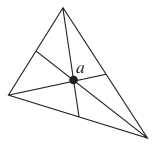
\includegraphics[width=0.20\textwidth]{img/tria_linear.png}\\
            \end{tabular}
            & $ R = O(h^2) $ & a & $ \frac{1}{3}, \frac{1}{3}, \frac{1}{3} $ & 1\\
        \hline
            Quadratic &
            \begin{tabular}{c}
                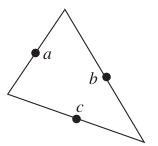
\includegraphics[width=0.20\textwidth]{img/tria_quadratic.png}
            \end{tabular}
            & $ R = O(h^3) $ & \begin{tabular}{c}
                a \\
                b \\
                c \\
            \end{tabular} & \begin{tabular}{c}
                $ \frac{1}{2}, \frac{1}{2} , 0 $ \\
                $ 0, \frac{1}{2}, \frac{1}{2} $ \\
                $ \frac{1}{2}, 0, \frac{1}{2} $ \\
            \end{tabular} & \begin{tabular}{c}
                $ \frac{1}{3} $ \\
                $ \frac{1}{3} $ \\
                $ \frac{1}{3} $ \\
            \end{tabular}\\
        \hline
            Cubic &
            \begin{tabular}{c}
                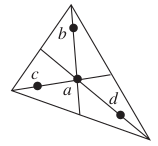
\includegraphics[width=0.20\textwidth]{img/tria_cubic.png}
            \end{tabular}
            & $ R = O(h^4) $ & \begin{tabular}{c}
                a \\
                b \\
                c \\
                d \\
            \end{tabular} & \begin{tabular}{c}
                $ \frac{1}{3}, \frac{1}{3} , \frac{1}{3} $ \\
                $ 0.6, 0.2, 0.2 $ \\
                $ 0.2, 0.6, 0.2 $ \\
                $ 0.2, 0.2, 0.6 $ \\
            \end{tabular} & \begin{tabular}{c}
                $ -\frac{27}{48} $ \\
                $ \frac{25}{48} $ \\
                $ \frac{25}{48} $ \\
                $ \frac{25}{48} $ \\
            \end{tabular}\\
        \hline
            Quintic &
            \begin{tabular}{c}
                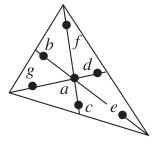
\includegraphics[width=0.20\textwidth]{img/tria_quintic.png}
            \end{tabular}
            & $ R = O(h^6) $ & \begin{tabular}{c}
                a \\
                b \\
                c \\
                d \\
                e \\
                f \\
                g \\
            \end{tabular} & \begin{tabular}{c}
                $ \frac{1}{3}, \frac{1}{3} , \frac{1}{3} $ \\
                $ \alpha_1, \beta_1, \beta_1 $ \\
                $ \beta_1, \alpha_1, \beta_1 $ \\
                $ \beta_1, \beta_1, \alpha_1 $ \\
                $ \alpha_2, \beta_2, \beta_2 $ \\
                $ \beta_2, \alpha_2, \beta_2 $ \\
                $ \beta_2, \beta_2, \alpha_2 $ \\
            \end{tabular} & \begin{tabular}{c}
                $ 0.225 000 000 0 $ \\
                $ 0.132 394 152 7 $ \\
                $ 0.132 394 152 7 $ \\
                $ 0.132 394 152 7 $ \\
                $ 0.125 939 180 5 $ \\
                $ 0.125 939 180 5 $ \\
                $ 0.125 939 180 5 $ \\
            \end{tabular}\\
            & & & \multicolumn{2}{l}{\begin{tabular}{l}
                with: \\
                $ \alpha_1 = $ 0.059 715 871 7 \\
                $ \beta_1 = $ 0.470 142 064 1 \\
                $ \alpha_2 = $ 0.797 426 985 3 \\
                $ \beta_2 = $ 0.101 286 507 3 \\
            \end{tabular}} & \\
        \hline
        \hline
    \end{tabular}}
    \caption{Triangular Element integration points and weights}
\end{table}


\newpage
\begin{table}[h!]
    \centering
    \renewcommand{\arraystretch}{1.25}
    % \small
    % \scriptsize
    \scalebox{0.80}{
    \begin{tabular}{||c c c c c c||}
        \hline
        \hline
        Order & Figure & Error & Points &
        \begin{tabular}{c} Tetrahedral\\Coordinates\end{tabular} & Weights\\
        \hline
            Linear &
            \begin{tabular}{c}
                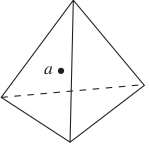
\includegraphics[width=0.20\textwidth]{img/tetra_linear.png}\\
            \end{tabular}
            & $ R = O(h^2) $ & a & $ \frac{1}{4}, \frac{1}{4}, \frac{1}{4}, \frac{1}{4} $ & 1\\
        \hline
            Quadratic &
            \begin{tabular}{c}
                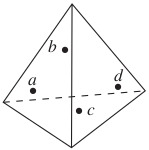
\includegraphics[width=0.20\textwidth]{img/tetra_quadratic.png}
            \end{tabular}
            & $ R = O(h^6) $ & \begin{tabular}{c}
                a \\
                b \\
                c \\
                d \\
            \end{tabular} & \begin{tabular}{c}
                $ \alpha, \beta, \beta, \beta $ \\
                $ \beta, \alpha, \beta, \beta $ \\
                $ \beta, \beta, \alpha, \beta $ \\
                $ \beta, \beta, \beta, \beta $ \\
            \end{tabular} & \begin{tabular}{c}
                $ \frac{1}{4} $ \\
                $ \frac{1}{4} $ \\
                $ \frac{1}{4} $ \\
                $ \frac{1}{4} $ \\
            \end{tabular}\\
            & & & \multicolumn{2}{l}{\begin{tabular}{l}
                with: \\
                $ \alpha = $ 0.585 410 20 \\
                $ \beta = $ 0.138 196 60 \\
            \end{tabular}} & \\
        \hline
            Cubic &
            \begin{tabular}{c}
                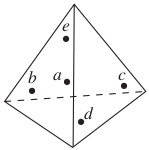
\includegraphics[width=0.20\textwidth]{img/tetra_cubic.png}
            \end{tabular}
            & $ R = O(h^4) $ & \begin{tabular}{c}
                a \\
                b \\
                c \\
                d \\
                e \\
            \end{tabular} & \begin{tabular}{c}
                $ \frac{1}{4}, \frac{1}{4}, \frac{1}{4}, \frac{1}{4} $ \\
                $ \frac{1}{2}, \frac{1}{6}, \frac{1}{6}, \frac{1}{6} $ \\
                $ \frac{1}{6}, \frac{1}{2}, \frac{1}{6}, \frac{1}{6} $ \\
                $ \frac{1}{6}, \frac{1}{6}, \frac{1}{2}, \frac{1}{6} $ \\
                $ \frac{1}{6}, \frac{1}{6}, \frac{1}{6}, \frac{1}{2} $ \\
            \end{tabular} & \begin{tabular}{c}
                $ -\frac{4}{5} $ \\
                $ \frac{9}{20} $ \\
                $ \frac{9}{20} $ \\
                $ \frac{9}{20} $ \\
                $ \frac{9}{20} $ \\
            \end{tabular}\\
        \hline
        \hline
    \end{tabular}}
    \caption{Tetrahedral Element integration points and weights}
\end{table}



\newpage
\section{General Element Matrices Procedure}
The procedure to generate any element stiffness, mass and load matrices can
be generalised to the following steps:

\begin{enumerate}
    \item Create Element domain in natural coordinates:
        \begin{itemize}
            \item $ -1 $ to $ 1 $ for quadrilateral elements
            \item $ 0 $ to $ 1 $ for triangular and linear elements
        \end{itemize}

    \item select the number of Gauss points based on the order of the element
        \begin{itemize}
            \item $ 2 $ for linear elements
            \item $ 3 $ for quadratic elements
        \end{itemize}

        Example:
        \begin{python}
import numpy as np
gp, gw = np.polynomial.legendre.leggauss(3)
        \end{python}

    \item Generate the shape functions $ \mathbf{N}_n^e $ in natural coordinates
        based on the number of Gauss points, dimension of the element and its domain.

        The $ \mathbf{N}_n^e $ matrix has the dimensions of:
        \begin{itemize}
            \item number of integration points = number of rows
            \item number of shape functions = number of columns
        \end{itemize}

        Therefore:

        \begin{equation}
            \mathbf{N}_n^e = \begin{bmatrix}
                N_{1,1}^e & \dots & N_{n,1}^e\\
                \vdots & \vdots & \vdots\\
                N_{1,m}^e & \dots & N_{n,m}^e
            \end{bmatrix}
        \end{equation}
         where $ 1 \dots m $ are the integration points and $ 1 \dots n $ are the shape
         functions.

    \item Transform the shape functions from natural coordinates to global coordinates
        \begin{eqarray}
            \mathbf{N}_g^e &= \mathbf{N}_n^e \mathbf{x}^e\\
            \mathbf{N}_g^e &= \begin{bmatrix}
                N_{1,1}^e(\xi) & \dots & N_{n,1}^e(\xi)\\
                \vdots & \vdots & \vdots\\
                N_{1,m}^e(\xi) & \dots & N_{n,m}^e(\xi)
            \end{bmatrix}
            \begin{bmatrix}
                x_1 & y_1 & z_1\\
                \vdots & \vdots & \vdots\\
                x_n & y_n & z_n
            \end{bmatrix}
        \end{eqarray}

        The $ \mathbf{x}^e $ matrix is a matrix of global coordinates of the element nodes.

        The resulting matrix has the dimension of:
        \begin{itemize}
            \item number of integration points = number of rows
            \item number of coordinates = number of columns (3D = 3, 2D = 2)
        \end{itemize}

    \item Generate the shape functions derivatives $ \mathbf{B}_n^e $
        in natural coordinates

        The shape functions derivatives matrix has 3 dimensions being
        \textit{number of integration points} $\times$ \textit{number of natural coordinates}
        $\times$ \textit{number of shape functions}

    \item Create the Matrix of Jacobians from the shape functions derivatives:
        \begin{equation}
            \mathbf{J} = \mathbf{B}_n^e \mathbf{x}^e
        \end{equation}

        The Matrix of Jacobians has the dimension of \textit{number of integration points}
        $\times$ \textit{number of global coordinates}
        $\times$ \textit{number of global coordinates}, where number of global coordinates
        means 2 for 2D and 3 for 3D problem.

    \item Get the Matrix of Jacobian determinants and an inverse Jacobian:
        \begin{equation}
            \mathbf{J}^{-1}\\
            \mathbf{J}_d = det \mathbf{J}
        \end{equation}

        Example:
        \begin{python}
d_jacobi = np.linalg.det(jacobi)
i_jacobi = np.linalg.inv(jacobi)
        \end{python}

        The Jacobian determinant is computed for each integration point and has a dimension
        of \textit{number of integration points} $\times$ \textit{1}

        The inverse Jacobian has the same dimension as the Jacobian (\textbf{must have})

    \item Transform the shape function derviatives from natural coordinates to
        global coordinates
        \begin{equation}
            \mathbf{B}_g^e = \mathbf{J}^{-1} \mathbf{B}_n^e
        \end{equation}

    \item Create the Material Stiffness matrix $ \mathbf{C} $

    \item Finally for each integration point:

        3D:
        \begin{eqarray}
            \mathbf{B}_{i,x}^e &= \textbf{B}_g(i, 0) \\
            \mathbf{B}_{i,y}^e &= \textbf{B}_g(i, 1) \\
            \mathbf{B}_{i,z}^e &= \textbf{B}_g(i, 2)\\
        \end{eqarray}

        where $ \mathbf{B}_{i,x}^e $,  $ \mathbf{B}_{i,y}^e $ and  $ \mathbf{B}_{i,z}^e $
        are vectors of legth = \textit{number of shape functions}

        Then matrix $ \mathbf{B} $ is:

        \begin{equation}
            \mathbf{B}_i = \begin{bmatrix}
                \textbf{B}_{i,x}^e & \mathbf{0} & \mathbf{0}\\
                \mathbf{0} & \textbf{B}_{i,y}^e & \mathbf{0}\\
                \mathbf{0} & \mathbf{0} & \textbf{B}_{i,z}^e \\
                \textbf{B}_{i,y}^e & \textbf{B}_{i,x}^e & \mathbf{0}\\
                \mathbf{0} & \textbf{B}_{i,z}^e & \textbf{B}_{i,y}^e \\
                \textbf{B}_{i,z}^e & \mathbf{0} & \textbf{B}_{i,x}^e
            \end{bmatrix}
        \end{equation}

        and matrix $ \mathbf{N} $ is:

        \begin{equation}
            \mathbf{N}_i = \begin{bmatrix}
                \textbf{N}_{n,i}^e & \mathbf{0} & \mathbf{0}\\
                \mathbf{0} & \textbf{N}_{n,i}^e & \mathbf{0}\\
                \mathbf{0} & \mathbf{0} & \textbf{N}_{n,i}^e
            \end{bmatrix}
        \end{equation}

        where $ \mathbf{0} $ is a zero vector of length = \textit{number of shape functions}
        and $ \mathbf{N}_{n,i}^e $ is a vector of shape functions in natural coordinates
        pertaining to the $i$-th integration point.

        Then:

        \begin{enumerate}
            \item \begin{equation}
                    \mathbf{K}_i^e = \mathbf{B}_i^T \mathbf{C} \mathbf{B}_i \ det \mathbf{J}_i
                    w_i
                  \end{equation}

            \item \begin{equation}
                    \mathbf{M}_i^e = \rho \mathbf{N}_i^T \mathbf{N}_i \ det \mathbf{J}_i
                    w_i
                  \end{equation}
            \item \begin{equation}
                    \mathbf{F}_i^e = \mathbf{N}_i^T \mathbf{F} \ det \mathbf{J}_i
                    w_i
                  \end{equation}

                  where $ \mathbf{F} = \begin{bmatrix}f_x \\ f_y \\ f_z\end{bmatrix} $
        \end{enumerate}

        where $ w_i $ is the multiple of gaussian weights for the respective
        integration point (for 3D case brick where the natural coordinates
        are $ \xi $, $ \eta $, $ \mu $ the $ w_i = w_{\xi_i} w_{\eta_i} w_{\mu_i} $

    \item Finally:
        \begin{enumerate}
            \item \begin{equation}
                    \mathbf{K}^e = \sum_{i=1}^n \mathbf{K}_i^e
                \end{equation}

            \item \begin{equation}
                    \mathbf{M}^e = \sum_{i=1}^n \mathbf{M}_i^e
                \end{equation}

            \item \begin{equation}
                    \mathbf{F}^e = \sum_{i=1}^n \mathbf{F}_i^e
                \end{equation}
        \end{enumerate}
\end{enumerate}



\newpage
\section{HEX8}

\subsection{Element Formulation}

The \textbf{Hexahedral} element is a 3-D quadrilateral \textbf{trilinear} element, otherwise known
as a \textbf{brick}. Topologically is hexahedron equivalent to a cube. It has eight
corners, twelve edges and six faces. Especially the \textbf{HEX8} element has
8 interpolation points.

\subsubsection{Natural coordinates}
The \textbf{natural coordinate system} of a hexahedral element are called
\textbf{isoparametric hexahedral coordinates}, denoted $ \xi $, $ \eta $ and $ \mu $.
The coordinates go from $ -1 $ to $ 1 $ and span from each face to the opposite one.
Each coordinate is 0 on the plane at midpoint of opposing faces called the
\textbf{median} face. This choice of limits is to facilitate the use of standard
\textit{Gauss integration formulas}.

\subsubsection{Corner Numbering Rules}
The eight corners of a hexahedron are locally numbered $ 1, 2, \dots , 8 $.
The corner numbering rule is:

\begin{itemize}
    \item select one face and numbers the corners of this face $ 1 \dots 4 $
          in a \textbf{counterclockwise} direction.
    \item number the corners directly opposite to corners $ 1, 2, 3, 4 $ as
          $ 5, 6, 7, 8 $ respectively.
\end{itemize}

The purpose of this numbering manner is so that a positive volume (or more
precisely, a positive \textbf{Jacobian determinant} at every point).

The definition of $ \xi $, $ \eta $ and $ \mu $ can be now made more precise:

\begin{itemize}
    \item $ \xi $ goes from $ -1 $ from (center of) face 1485 to $ +1 $ on face 2376
    \item $ \eta $ goes from $ -1 $ from (center of) face 1265 to $ +1 $ on face 3487
    \item $ \mu $ goes from $ -1 $ from (center of) face 1234 to $ +1 $ on face 5678
\end{itemize}

\begin{figure}[ht]
    \centering
    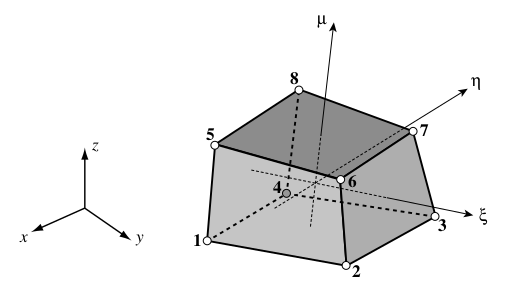
\includegraphics[width=0.90\textwidth]{img/hex8-node-numbers.png}
    \caption{The 8-node hexahedron and the natural coordinates $ \eta $, $ \xi $
    and $ \mu $.}
    \label{fig:hex8-node-numbers-png}
\end{figure}


\subsubsection{Element Definition}

The 8-noded hexahedral element is defined by:

\begin{eqarray}
    \begin{bmatrix}
        1\\
        x\\
        y\\
        z\\
        u_x\\
        u_y\\
        u_z
    \end{bmatrix} &=
    \begin{bmatrix}
        1 & 1 & 1 & 1 & 1 & 1 & 1 & 1\\
        x_1 & x_2 & x_3 & x_4 & x_5 & x_6 & x_7 & x_8\\
        y_1 & y_2 & y_3 & y_4 & y_5 & y_6 & y_7 & y_8\\
        y_1 & y_2 & y_3 & y_4 & y_5 & y_6 & y_7 & y_8\\
        u_{x1} & u_{x2} & u_{x3} & u_{x4} & u_{x5} & u_{x6} & u_{x7} & u_{x8}\\
        u_{y1} & u_{y2} & u_{y3} & u_{y4} & u_{y5} & u_{y6} & u_{y7} & u_{y8}\\
        u_{z1} & u_{z2} & u_{z3} & u_{z4} & u_{z5} & u_{z6} & u_{z7} & u_{z8}
    \end{bmatrix}
    \begin{bmatrix}
        N_1^e\\
        N_2^e\\
        N_3^e\\
        N_4^e\\
        N_5^e\\
        N_6^e\\
        N_7^e\\
        N_8^e
    \end{bmatrix}
\end{eqarray}

The hexahedron corners natural coordinates are:

\begin{table}[ht]
    \centering
    \begin{tabular}{|c c c c|}
        \hline
        node & $\xi$ & $\eta$ & $\mu$\\
        \hline
        1 & -1 & -1 & -1\\
        2 & +1 & -1 & -1\\
        3 & +1 & +1 & -1\\
        4 & -1 & +1 & -1\\
        5 & -1 & -1 & +1\\
        6 & +1 & -1 & +1\\
        7 & +1 & +1 & +1\\
        8 & -1 & +1 & +1\\
        \hline
    \end{tabular}\\
    \caption{Hexahedron corners natural coordinates}
\end{table}

The shape functions are:
\begin{eqarray}
    N_1^e &= \frac{1}{8} \left(1-\xi\right) \left(1-\eta\right) \left(1-\mu\right)\\
    N_2^e &= \frac{1}{8} \left(1+\xi\right) \left(1-\eta\right) \left(1-\mu\right)\\
    N_3^e &= \frac{1}{8} \left(1+\xi\right) \left(1+\eta\right) \left(1-\mu\right)\\
    N_4^e &= \frac{1}{8} \left(1-\xi\right) \left(1+\eta\right) \left(1-\mu\right)\\
    N_5^e &= \frac{1}{8} \left(1-\xi\right) \left(1-\eta\right) \left(1+\mu\right)\\
    N_6^e &= \frac{1}{8} \left(1+\xi\right) \left(1-\eta\right) \left(1+\mu\right)\\
    N_7^e &= \frac{1}{8} \left(1+\xi\right) \left(1+\eta\right) \left(1+\mu\right)\\
    N_8^e &= \frac{1}{8} \left(1-\xi\right) \left(1+\eta\right) \left(1+\mu\right)
\end{eqarray}

\begin{bbox}[0.96]
    The eight formulas can be summarised in a single expression:

    \begin{equation}
        N_i^e = \frac{1}{8}
              \left(1+\xi\xi_i\right)
              \left(1+\eta\eta_i\right)
              \left(1+\mu\mu_i\right)
    \end{equation}

    where $\xi_i$, $\eta_i$ and $\mu_i$ denote the coordinates of the $i$-th node.
\end{bbox}


\subsubsection{Partial Derivatives}
The calculation of the shape functions derivatives with respect to the natural
coordinates:

\begin{eqarray}
    \frac{\partial N_1^e}{\partial\xi} &= -\frac{1}{8} \left(1-\eta\right) \left(1-\mu\right)\\
    \frac{\partial N_2^e}{\partial\xi} &= \frac{1}{8} \left(1-\eta\right) \left(1-\mu\right)\\
    \frac{\partial N_3^e}{\partial\xi} &= \frac{1}{8} \left(1+\eta\right) \left(1-\mu\right)\\
    \frac{\partial N_4^e}{\partial\xi} &= -\frac{1}{8} \left(1+\eta\right) \left(1-\mu\right)\\
    \frac{\partial N_5^e}{\partial\xi} &= -\frac{1}{8} \left(1-\eta\right) \left(1+\mu\right)\\
    \frac{\partial N_6^e}{\partial\xi} &= \frac{1}{8} \left(1-\eta\right) \left(1+\mu\right)\\
    \frac{\partial N_7^e}{\partial\xi} &= \frac{1}{8} \left(1+\eta\right) \left(1+\mu\right)\\
    \frac{\partial N_8^e}{\partial\xi} &= -\frac{1}{8} \left(1+\eta\right) \left(1+\mu\right)
\end{eqarray}

\begin{eqarray}
    \frac{\partial N_1^e}{\partial\eta} &= -\frac{1}{8} \left(1-\xi\right) \left(1-\mu\right)\\
    \frac{\partial N_2^e}{\partial\eta} &= -\frac{1}{8} \left(1+\xi\right) \left(1-\mu\right)\\
    \frac{\partial N_3^e}{\partial\eta} &= \frac{1}{8} \left(1+\xi\right) \left(1-\mu\right)\\
    \frac{\partial N_4^e}{\partial\eta} &= \frac{1}{8} \left(1-\xi\right) \left(1-\mu\right)\\
    \frac{\partial N_5^e}{\partial\eta} &= -\frac{1}{8} \left(1-\xi\right) \left(1+\mu\right)\\
    \frac{\partial N_6^e}{\partial\eta} &= -\frac{1}{8} \left(1+\xi\right) \left(1+\mu\right)\\
    \frac{\partial N_7^e}{\partial\eta} &= \frac{1}{8} \left(1+\xi\right) \left(1+\mu\right)\\
    \frac{\partial N_8^e}{\partial\eta} &= \frac{1}{8} \left(1-\xi\right) \left(1+\mu\right)
\end{eqarray}

\begin{eqarray}
    \frac{\partial N_1^e}{\partial\mu} &= -\frac{1}{8} \left(1-\xi\right) \left(1-\eta\right)\\
    \frac{\partial N_2^e}{\partial\mu} &= -\frac{1}{8} \left(1+\xi\right) \left(1-\eta\right)\\
    \frac{\partial N_3^e}{\partial\mu} &= -\frac{1}{8} \left(1+\xi\right) \left(1+\eta\right)\\
    \frac{\partial N_4^e}{\partial\mu} &= -\frac{1}{8} \left(1-\xi\right) \left(1+\eta\right)\\
    \frac{\partial N_5^e}{\partial\mu} &= \frac{1}{8} \left(1-\xi\right) \left(1-\eta\right)\\
    \frac{\partial N_6^e}{\partial\mu} &= \frac{1}{8} \left(1+\xi\right) \left(1-\eta\right)\\
    \frac{\partial N_7^e}{\partial\mu} &= \frac{1}{8} \left(1+\xi\right) \left(1+\eta\right)\\
    \frac{\partial N_8^e}{\partial\mu} &= \frac{1}{8} \left(1-\xi\right) \left(1+\eta\right)
\end{eqarray}

\begin{bbox}
    \textbf{Note:}

    The partial derivatives can be also written as:

    \begin{eqarray}
        \frac{\partial N_i^e}{\partial \xi} &= \frac{1}{8} \frac{\xi_i}{|\xi_i|}
            \left(1+\eta\eta_i\right) \left(1+\mu\mu_i\right) \\
        \frac{\partial N_i^e}{\partial \eta} &= \frac{1}{8} \frac{\eta_i}{|\eta_i|}
            \left(1+\xi\xi_i\right) \left(1+\mu\mu_i\right) \\
        \frac{\partial N_i^e}{\partial \mu} &= \frac{1}{8} \frac{\mu_i}{|\mu_i|}
            \left(1+\xi\xi_i\right) \left(1+\eta\eta_i\right)
    \end{eqarray}
\end{bbox}



\textbf{The Jacobian:}

The derivatives of the shape functions are given by the usual chain rule formulas:

\begin{eqarray}
    \frac{\partial N_i^e}{\partial x} &=
        \frac{\partial N_i^e}{\partial \xi} \frac{\partial \xi}{\partial x} +
        \frac{\partial N_i^e}{\partial \eta} \frac{\partial \eta}{\partial x} +
        \frac{\partial N_i^e}{\partial \mu} \frac{\partial \mu}{\partial x}\\
    \frac{\partial N_i^e}{\partial y} &=
        \frac{\partial N_i^e}{\partial \xi} \frac{\partial \xi}{\partial y} +
        \frac{\partial N_i^e}{\partial \eta} \frac{\partial \eta}{\partial y} +
        \frac{\partial N_i^e}{\partial \mu} \frac{\partial \mu}{\partial y}\\
    \frac{\partial N_i^e}{\partial z} &=
        \frac{\partial N_i^e}{\partial \xi} \frac{\partial \xi}{\partial z} +
        \frac{\partial N_i^e}{\partial \eta} \frac{\partial \eta}{\partial z} +
        \frac{\partial N_i^e}{\partial \mu} \frac{\partial \mu}{\partial z}
\end{eqarray}

In matrix form:

\begin{eqarray}
    \begin{bmatrix}
        \frac{\partial N_i^e}{\partial x}\\
        \frac{\partial N_i^e}{\partial y}\\
        \frac{\partial N_i^e}{\partial z}
    \end{bmatrix} &=
    \begin{bmatrix}
        \frac{\partial \xi}{\partial x} &
        \frac{\partial \eta}{\partial x} &
        \frac{\partial \mu}{\partial x}\\
        \frac{\partial \xi}{\partial y} &
        \frac{\partial \eta}{\partial y} &
        \frac{\partial \mu}{\partial y}\\
        \frac{\partial \xi}{\partial z} &
        \frac{\partial \eta}{\partial z} &
        \frac{\partial \mu}{\partial z}
    \end{bmatrix}
    \begin{bmatrix}
        \frac{\partial N_i^e}{\partial \xi}\\
        \frac{\partial N_i^e}{\partial \eta}\\
        \frac{\partial N_i^e}{\partial \mu}
    \end{bmatrix}
\end{eqarray}

The $ 3 \times 3 $ matrix above is $ \mathbf{J}^{-1} $, the inverse of:
\begin{eqarray}
    \mathbf{J} = \frac{\partial \left( x, y, z \right)}{\partial \left( \xi, \eta, \mu \right)}
    = \begin{bmatrix}
        \frac{\partial x}{\partial \xi} &
        \frac{\partial y}{\partial \xi} &
        \frac{\partial z}{\partial \xi} \\
        \frac{\partial x}{\partial \eta} &
        \frac{\partial y}{\partial \eta} &
        \frac{\partial z}{\partial \eta} \\
        \frac{\partial x}{\partial \mu} &
        \frac{\partial y}{\partial \mu} &
        \frac{\partial z}{\partial \mu}
    \end{bmatrix}
\end{eqarray}

Matrix $ \mathbf{J} $ is called the \textit{Jacobian matrix} of $ (x, y, z) $
with respect to $ (\xi, \eta, \mu) $. In the finite element literature, matrices
$ \mathbf{J} $ and $ \mathbf{J}^{-1} $ are called simply the \textit{Jacobian} and
\textit{inverse Jacobian}, respectively, although such a short name us sometimes
ambiguous. The notation

\begin{eqarray}
    \mathbf{J} &=
    \frac{\partial \left(x, y, z \right)}{\partial \left(\xi, \eta, \mu \right)}\\
    \mathbf{J}^{-1} &=
    \frac{\partial \left(\xi, \eta, \mu \right)}{\partial \left(x, y, z \right)}
\end{eqarray}

is standard in multivariable calculus and suggests that the Jacobian may be viewed as
a generalisation of the ordinary derivativem to which it reduces for a scalar
function $ \mathbf{x} = x(\xi) $.



\subsubsection{Computing the Jacobian Matrix}
The isoparametric definitioin of hexahedron element geometry is:

\begin{eqarray}
    x &= x_i N_i^e\\
    y &= y_i N_i^e\\
    z &= z_i N_i^e
\end{eqarray}

where the summation convention is understood to apply over $ i = 1, 2, \dots , n $,
in which $ n $ denotes the number of element nodes.

\begin{bbox}
    \textbf{Note:} This for a given hexahedral element gives an $ n \times 3 $ matrix.
\end{bbox}


Differentiating these relations with respect to the hexahedron coordinates we construct
the matrix $ \mathbf{J} $ as follows:

\begin{equation}
    \mathbf{J} =
    \begin{bmatrix}
        x_i \frac{\partial N_i^e}{\partial \xi} &
        y_i \frac{\partial N_i^e}{\partial \xi} &
        z_i \frac{\partial N_i^e}{\partial \xi}\\
        x_i \frac{\partial N_i^e}{\partial \eta} &
        y_i \frac{\partial N_i^e}{\partial \eta} &
        z_i \frac{\partial N_i^e}{\partial \eta}\\
        x_i \frac{\partial N_i^e}{\partial \mu} &
        y_i \frac{\partial N_i^e}{\partial \mu} &
        z_i \frac{\partial N_i^e}{\partial \mu}
    \end{bmatrix}
\end{equation}

or:
\begin{equation}
    \mathbf{J}_i =
    \begin{bmatrix}
        \frac{\partial N_1^e}{\partial \xi} &
        \frac{\partial N_2^e}{\partial \xi} &
        \dots &
        \frac{\partial N_n^e}{\partial \xi}\\
        \frac{\partial N_1^e}{\partial \eta} &
        \frac{\partial N_2^e}{\partial \eta} &
        \dots &
        \frac{\partial N_n^e}{\partial \eta}\\
        \frac{\partial N_1^e}{\partial \mu} &
        \frac{\partial N_2^e}{\partial \mu} &
        \dots &
        \frac{\partial N_n^e}{\partial \mu}
    \end{bmatrix}
    \begin{bmatrix}
        x_1 & y_1 & z_1 \\
        x_2 & y_2 & z_2 \\
        \vdots & \vdots & \vdots \\
        x_n & y_n & z_n
    \end{bmatrix}
\end{equation}


Given a point of hexahedron coordinates $ ( \xi, \eta, \mu ) $ the Jacobian $ \mathbf{J} $
can be easilly formed using the above formula, and numerically inverted to form
$ \mathbf{J}^{-1} $.


\subsubsection{The Strain-Displacement Matrix}

Having obtained the shape function derivatives, the matrix $ \mathbf{B} $ for hexahedron
element displays the usual structure for 3D elements:

\begin{equation}
    \mathbf{B} = \mathbf{D}\mathbf{\Phi} =
    \begin{bmatrix}
        \frac{\partial}{\partial x} & 0 & 0 \\
        0 & \frac{\partial}{\partial y} & 0 \\
        0 & 0 & \frac{\partial}{\partial z} \\
        \frac{\partial}{\partial y} & \frac{\partial}{\partial x} & 0 \\
        0 & \frac{\partial}{\partial z} & \frac{\partial}{\partial y} \\
        \frac{\partial}{\partial z} & 0 & \frac{\partial}{\partial x}
    \end{bmatrix}
    \begin{bmatrix}
        \mathbf{q} & \mathbf{0} & \mathbf{0} \\
        \mathbf{0} & \mathbf{q} & \mathbf{0} \\
        \mathbf{0} & \mathbf{0} & \mathbf{q}
    \end{bmatrix} =
    \begin{bmatrix}
        \mathbf{q}_x & \mathbf{0} & \mathbf{0} \\
        \mathbf{0} & \mathbf{q}_y & \mathbf{0} \\
        \mathbf{0} & \mathbf{0} & \mathbf{q}_z \\
        \mathbf{q}_y & \mathbf{q}_x & \mathbf{0} \\
        \mathbf{0} & \mathbf{q}_z & \mathbf{q}_y \\
        \mathbf{q}_z & \mathbf{0} & \mathbf{q}_x
    \end{bmatrix}
\end{equation}

where:
\begin{eqarray}
    \mathbf{q} &= \begin{bmatrix} N_1^e & \dots & N_n^e \end{bmatrix}\\
    \mathbf{q}_x &= \begin{bmatrix} \frac{\partial N_1^e}{\partial x} & \dots & \frac{\partial N_n^e}{\partial x} \end{bmatrix}\\
    \mathbf{q}_y &= \begin{bmatrix} \frac{\partial N_1^e}{\partial y} & \dots & \frac{\partial N_n^e}{\partial y} \end{bmatrix}\\
    \mathbf{q}_z &= \begin{bmatrix} \frac{\partial N_1^e}{\partial z} & \dots & \frac{\partial N_n^e}{\partial z} \end{bmatrix}
\end{eqarray}

are row vectors of length $ n $, $ n $ being the number of nodes in the element.



\subsubsection{Stiffness Matrix Evaluation}

The element stiffness Matrix is given by:

\begin{equation}
    \mathbf{K}^e = \int_{V^e} \mathbf{B}^T \mathbf{E} \mathbf{B} dV^e
\end{equation}

As in two-dimensional case, this is replaced by a numerical integration formula which
now involves a triple loop over conventional Gauss quadrature rules. Assuming that
the stress-strain matrix $ \mathbf{E} $ is constant over the element,

\begin{equation}
    \mathbf{K}^e = \sum_{i=1}^{p_1} \sum_{j=1}^{p_2} \sum_{k=1}^{p_3}
    w_i w_j w_k \mathbf{B}_{ijk}^T \mathbf{E} \mathbf{B}_{ijk} \mathbf{J}_{ijk}
\end{equation}

Here $ p_1 $, $ p_2 $ and $ p_3 $ are the number of Gauss points in the $ \xi $,
$ \eta $ and $ \mu $ direction, respectively, while $ \mathbf{B}_{ijk} $
and $ \mathbf{J}_{ijk} $ are abbreviations for:

\begin{eqarray}
    \mathbf{B}_{ijk} &= \mathbf{B} \left(\xi_i, \eta_i, \mu_i\right) \\
    \mathbf{J}_{ijk} &= det \mathbf{J} \left(\xi_i, \eta_i, \mu_i\right)
\end{eqarray}

Usually the number of integration points is taken the same in all directions:
$ p = p_1 = p_2 = p_3 $. The total number of Gauss points is thus $ p^3 $.
Each point adds at most 6 to the stiffness matrix rank. The minimum rank-sufficient
rules for the 8-node and 20-node hexahedra are $ p = 2 $ and $ p = 3 $, respectively.


\subsection{Python implementation}

\begin{python}
#!/usr/bin/python3

import numpy as np
np.set_printoptions(precision=2) # , suppress=True)

def hex8_stiffness_mass_load(coors: np.ndarray,
                             E: float,
                             nu: float,
                             rho: float,
                             fx: float = 0.,
                             fy: float = 0.,
                             fz: float = 0.):
    """
    In:
        coors - 8 x 3 coordinate matrix
                [[x1,y1,z1], ... , [xn,yn,zn]
        E     - Youngs's Modulus
        nu    - Poisson's Constant
        rho   - Density
        fx    - Volumetric Load in x direction
        fy    - Volumetric Load in y direction
        fz    - Volumetric Load in z direction
    """
    domain = np.array([[-1., -1., -1.],
                       [1., -1., -1.],
                       [1., 1., -1.],
                       [-1., 1., -1.],
                       [-1., -1., 1.],
                       [1., -1., 1.],
                       [1., 1., 1.],
                       [-1., 1., 1.]], dtype=float)
    print('Domain: {0}\n{1}'.format(domain.shape, domain))

    # gaussian interpolation
    gauss_points = 3
    g_points, g_weights = np.polynomial.legendre.leggauss(gauss_points)
    integration_points = []
    interpolation_weights = []
    for i, xi in enumerate(g_points):
        for j, eta in enumerate(g_points):
            for k, mu in enumerate(g_points):
                integration_points.append([xi, eta, mu])
                interpolation_weights.append(g_weights[i] *
                                             g_weights[j] *
                                             g_weights[k])
    integration_points = np.array(integration_points, dtype=float)
    interpolation_weights = np.array(interpolation_weights, dtype=float)
    print('Gauss Integration '
          '{0}:\n{1}\nWeights:\n{2}'.format(gauss_points,
                                            integration_points,
                                            interpolation_weights))

    full_domain = np.vstack((domain, integration_points))

    # Shape Functions in Natural Coordinates
    xi = integration_points.T[0]
    eta = integration_points.T[1]
    mu = integration_points.T[2]
    psi = np.zeros((8, integration_points.shape[0]), dtype=float)
    for i in range(8):
        psi[i] = 1/8 * (1 + xi * domain[i, 0]) *
                       (1 + eta * domain[i, 1]) *
                       (1 + mu * domain[i, 2])
    psi = psi.T
    print('Shape Functions: {0}\n{1}'.format(psi.shape, psi))

    # Shape Functions in Global Coordinates
    psi_g = psi @ coors
    print('Shape Functions in '
          'Global Coordinates: {0}\n{1}'.format(psi_g.shape, psi_g))

    # Shape Functions Derivatives in Natural Coordinates
    dpsi = 1 / 8 * np.array([[(eta - 1.0) * (1.0 - mu),# 1
                              (xi - 1) * (1 - mu),
                             -(1 - xi) * (1 - eta)],
                             [(1 - eta) * (1 - mu),    # 2
                              (-1 - xi) * (1 - mu),
                             -(1 + xi) * (1 - eta)],
                             [(1 + eta) * (1 - mu),    # 3
                              (1 + xi) * (1 - mu),
                             -(1 + xi) * (1 + eta)],
                             [(-1.0 - eta) * (1 - mu), # 4
                              (1 - xi) * (1 - mu),
                             -(1 - xi) * (1 + eta)],
                             [(1 - eta) * (-1 - mu),   # 5
                             -(1 - xi) * (1 + mu),
                              (1 - xi) * (1 - eta)],
                             [(1 - eta) * (1 + mu),    # 6
                             -(1 + xi) * (1 + mu),
                              (1 + xi) * (1 - eta)],
                             [(1 + eta) * (1 + mu),    # 7
                              (1 + xi) * (1 + mu),
                              (1 + xi) * (1 + eta)],
                             [-(1 + eta) * (1 + mu),   # 8
                              (1 - xi) * (1 + mu),
                              (1 - xi) * (1 + eta)]])
    dpsi = dpsi.T
    print('Shape Functions Derivatives: '
          '{0}\n{1}'.format(dpsi.shape, dpsi))

    # Jacobian Matrix
    jacobi = dpsi @ coors
    print('Jacobian Matrix: {0}\n{1}'.format(jacobi.shape, jacobi))

    # Jacobian Determinants
    d_jacobi = np.linalg.det(jacobi)
    print('Determinant of Jacobian: '
          '{0}\n{1}'.format(d_jacobi.shape, d_jacobi))

    # Inverse Jacobian
    i_jacobi = np.linalg.inv(jacobi)
    print('Inverse Jacobian Matrix: '
          '{0}\n{1}'.format(i_jacobi.shape, i_jacobi))

    # Shape Function Derivatives in Global Coordinates
    dpsi_g = i_jacobi @ dpsi
    print('Shape Function Derivatives in Global Coordinates: '
          '{0}\n{1}'.format(dpsi_g.shape, dpsi_g))

    # Material Stiffness Matrix
    C = E / ((1.0 + nu) * (1.0 - 2.0 * nu)) *
        np.array([[1.0 - nu, nu, nu, 0.0, 0.0, 0.0],
                  [nu, 1.0 - nu, nu, 0.0, 0.0, 0.0],
                  [nu, nu, 1.0 - nu, 0.0, 0.0, 0.0],
                  [0.0, 0.0, 0.0, (1.0 - 2.0 * nu) / 2.0, 0.0, 0.0],
                  [0.0, 0.0, 0.0, 0.0, (1.0 - 2.0 * nu) / 2.0, 0.0],
                  [0.0, 0.0, 0.0, 0.0, 0.0, (1.0 - 2.0 * nu) / 2.0]],
                  dtype=float)
    print('Material Stiffness Matrix: {0}\n{1}'.format(C.shape, C))

    # Create Element Stiffness and Mass Matrix
    Ke = np.zeros((domain.size, domain.size), dtype=float)
    Me = np.zeros((domain.size, domain.size), dtype=float)
    Fe = np.zeros((domain.size, 1), dtype=float)
    # o = np.zeros(domain.shape[0], dtype=float)

    # iterate over Gauss points of domain, * means unpack values
    for i in range(integration_points.shape[0]):
        # this is smart but arranges dofs by component, not by node
        # component-wise dof ordering (x1, .. , y1, .. y4, z1, .. , z4)
        # B = np.array([
        #   [*dpsi_g[i, 0, :], *o, *o],
        #   [*o, *dpsi_g[i, 1, :], *o],
        #   [*o, *o, *dpsi_g[i, 2, :]],
        #   [*dpsi_g[i, 2, :], *o, *dpsi_g[i, 0, :]],
        #   [*o, *dpsi_g[i, 2, :], *dpsi_g[i, 1, :]],
        #   [*dpsi_g[i, 1, :], *dpsi_g[i, 0, :], *o]], dtype=float)

        # dofs ordered by node
        # node wise dof ordering (x1, y1, z1, .. , x4, y4, z4)
        dpx = dpsi_g[i,0,:]
        dpy = dpsi_g[i,1,:]
        dpz = dpsi_g[i,2,:]
        B = np.array(
            [[dpx[0],0,0,dpx[1],0,0,dpx[2],0,0,dpx[3],0,0],
             [0,dpy[0],0,0,dpy[1],0,0,dpy[2],0,0,dpy[3],0],
             [0,0,dpz[0],0,0,dpz[1],0,0,dpz[2],0,0,dpz[3]],
             [dpy[0],dpx[0],0,dpy[1],dpx[1],0,dpy[2],dpx[2],0,dpy[3],dpx[3],0],
             [0,dpz[0],dpy[0],0,dpz[1],dpy[1],0,dpz[2],dpy[2],0,dpz[3],dpy[3]],
             [dpz[0],0,dpx[0],dpz[1],0,dpx[1],dpz[2],0,dpx[2],dpz[3],0,dpx[3]],
             dtype=float)

        # component-wise dof ordering (x1, .. , y1, .. y4, z1, .. , z4)
        # N = np.array([[*psi[i], *o, *o],
        #               [*o, *psi[i], *o],
        #               [*o, *o, *psi[i]]], dtype=float)

        # node wise dof ordering (x1, y1, z1, .. , x4, y4, z4)
        N = np.array([[psi[i,0],0,0,psi[i,1],0,0,psi[i,2],0,0,psi[i,3],0,0],
                      [0,psi[i,0],0,0,psi[i,1],0,0,psi[i,2],0,0,psi[i,3],0],
                      [0,0,psi[i,0],0,0,psi[i,1],0,0,psi[i,2],0,0,psi[i,3]],
                      dtype=float)

        F = np.array([[fx], [fy], [fz]], dtype=float)

        Ke += (B.T @ C @ B) * d_jacobi[i] * interpolation_weights[i]
        Me += rho * (N.T @ N) * d_jacobi[i] * interpolation_weights[i]
        Fe += (N.T @ F) * d_jacobi[i] * interpolation_weights[i]

    print('Element Stiffness Matrix: {0}\n{1}'.format(Ke.shape, Ke))
    print('Element Mass Matrix: {0}\n{1}'.format(Me.shape, Me))
    print('Element Volume Force Vector: {0}\n{1}'.format(Fe.shape, Fe))
\end{python}

And to get stresses:
\begin{python}
#!/usr/bin/python3

import numpy as np
np.set_printoptions(precision=2) # , suppress=True)

def hex8_stresses(coors: np.ndarray,
                  disp: np.ndarray,
                  E: float,
                  nu: float):
    """
    In:
        coors - 8 x 3 coordinate matrix
                [[x1,y1,z1], ... , [xn,yn,zn]
        disp  - 8 x 3 coordinate matrix
                [[u1,v1,w1], ... , [un,vn,wn]
        E     - Youngs's Modulus
        nu    - Poisson's Constant
    """
    domain = np.array([[-1., -1., -1.],
                       [1., -1., -1.],
                       [1., 1., -1.],
                       [-1., 1., -1.],
                       [-1., -1., 1.],
                       [1., -1., 1.],
                       [1., 1., 1.],
                       [-1., 1., 1.]], dtype=float)
    print('Domain: {0}\n{1}'.format(domain.shape, domain))

    # gaussian interpolation
    gauss_points = 3
    g_points, g_weights = np.polynomial.legendre.leggauss(gauss_points)
    integration_points = []
    interpolation_weights = []
    for i, xi in enumerate(g_points):
        for j, eta in enumerate(g_points):
            for k, mu in enumerate(g_points):
                integration_points.append([xi, eta, mu])
                interpolation_weights.append(g_weights[i] *
                                             g_weights[j] *
                                             g_weights[k])
    integration_points = np.array(integration_points, dtype=float)
    interpolation_weights = np.array(interpolation_weights, dtype=float)
    print('Gauss Integration '
          '{0}:\n{1}\nWeights:\n{2}'.format(gauss_points,
                                            integration_points,
                                            interpolation_weights))

    full_domain = np.vstack((domain, integration_points))

    # Shape Functions in Natural Coordinates
    xi = integration_points.T[0]
    eta = integration_points.T[1]
    mu = integration_points.T[2]
    psi = np.zeros((8, integration_points.shape[0]), dtype=float)
    for i in range(8):
        psi[i] = 1/8 * (1 + xi * domain[i, 0]) *
                       (1 + eta * domain[i, 1]) *
                       (1 + mu * domain[i, 2])
    psi = psi.T
    print('Shape Functions: {0}\n{1}'.format(psi.shape, psi))

    # Shape Functions in Global Coordinates
    psi_g = psi @ coors
    print('Shape Functions in '
          'Global Coordinates: {0}\n{1}'.format(psi_g.shape, psi_g))

    # Shape Functions Derivatives in Natural Coordinates
    dpsi = 1 / 8 * np.array([[(eta - 1.0) * (1.0 - mu),# 1
                              (xi - 1) * (1 - mu),
                             -(1 - xi) * (1 - eta)],
                             [(1 - eta) * (1 - mu),    # 2
                              (-1 - xi) * (1 - mu),
                             -(1 + xi) * (1 - eta)],
                             [(1 + eta) * (1 - mu),    # 3
                              (1 + xi) * (1 - mu),
                             -(1 + xi) * (1 + eta)],
                             [(-1.0 - eta) * (1 - mu), # 4
                              (1 - xi) * (1 - mu),
                             -(1 - xi) * (1 + eta)],
                             [(1 - eta) * (-1 - mu),   # 5
                             -(1 - xi) * (1 + mu),
                              (1 - xi) * (1 - eta)],
                             [(1 - eta) * (1 + mu),    # 6
                             -(1 + xi) * (1 + mu),
                              (1 + xi) * (1 - eta)],
                             [(1 + eta) * (1 + mu),    # 7
                              (1 + xi) * (1 + mu),
                              (1 + xi) * (1 + eta)],
                             [-(1 + eta) * (1 + mu),   # 8
                              (1 - xi) * (1 + mu),
                              (1 - xi) * (1 + eta)]])
    dpsi = dpsi.T
    print('Shape Functions Derivatives: '
          '{0}\n{1}'.format(dpsi.shape, dpsi))

    # Jacobian Matrix
    jacobi = dpsi @ coors
    print('Jacobian Matrix: {0}\n{1}'.format(jacobi.shape, jacobi))

    # Jacobian Determinants
    d_jacobi = np.linalg.det(jacobi)
    print('Determinant of Jacobian: '
          '{0}\n{1}'.format(d_jacobi.shape, d_jacobi))

    # Inverse Jacobian
    i_jacobi = np.linalg.inv(jacobi)
    print('Inverse Jacobian Matrix: '
          '{0}\n{1}'.format(i_jacobi.shape, i_jacobi))

    # Shape Function Derivatives in Global Coordinates
    dpsi_g = i_jacobi @ dpsi
    print('Shape Function Derivatives in Global Coordinates: '
          '{0}\n{1}'.format(dpsi_g.shape, dpsi_g))

    # Material Stiffness Matrix
    C = E / ((1.0 + nu) * (1.0 - 2.0 * nu)) *
        np.array([[1.0 - nu, nu, nu, 0.0, 0.0, 0.0],
                  [nu, 1.0 - nu, nu, 0.0, 0.0, 0.0],
                  [nu, nu, 1.0 - nu, 0.0, 0.0, 0.0],
                  [0.0, 0.0, 0.0, (1.0 - 2.0 * nu) / 2.0, 0.0, 0.0],
                  [0.0, 0.0, 0.0, 0.0, (1.0 - 2.0 * nu) / 2.0, 0.0],
                  [0.0, 0.0, 0.0, 0.0, 0.0, (1.0 - 2.0 * nu) / 2.0]],
                  dtype=float)
    print('Material Stiffness Matrix: {0}\n{1}'.format(C.shape, C))

    du = disp.T @ np.transpose(dpsi_g, axes=[0, 2, 1])

    exx = du[:, 0, 0]
    eyy = du[:, 1, 1]
    ezz = du[:, 2, 2]
    exy = du[:, 0, 1] + du[:, 1, 0]
    eyz = du[:, 1, 2] + du[:, 2, 1]
    exz = du[:, 0, 2] + du[:, 2, 0]
    epsilons = np.array([exx, eyy, ezz, exy, eyz, exz])

    sigmas = (C @ epsilons).T
    epsilons = epsilons.T
    print('Element Strains: {0}\n{1}'.format(epsilons.shape, epsilons))
    print('Element Stresses: {0}\n{1}'.format(stresses.shape, stresses))
\end{python}




\newpage
\section{TET4 Element}

\subsection{Element Formulation}


\subsection{Python Implementation}
\begin{python}
#!/usr/bin/python3

import numpy as np
np.set_printoptions(precision=2) # , suppress=True)

def tet4_stiffness_mass_load(coors: np.ndarray,
                             E: float,
                             nu: float,
                             rho: float,
                             fx: float = 0.,
                             fy: float = 0.,
                             fz: float = 0.,
                             gauss_points = 4):
    domain = np.array([[1., 0., 0., 0.],
                       [0., 1., 0., 0.],
                       [0., 0., 1., 0.],
                       [0., 0., 0., 1.]], dtype=float)
    print('Domain: {0}\n{1}'.format(domain.shape, domain))

    # gaussian interpolation
    integration_points = None
    integration_weights = None
    if gauss_points == 1:
        integration_points = np.array([1/4, 1/4, 1/4, 1/4],
                                      dtype=float).reshape(1, 4)
        integration_weights = np.array([1 * 1 * 1 * 1],
                                       dtype=float) * 1/6

    elif gauss_points == 4:
        a = 0.58541020
        b = 0.13819660
        integration_points = np.array([[a, b, b, b],
                                       [b, a, b, b],
                                       [b, b, a, b],
                                       [b, b, b, a]], dtype=float)
        integration_weights = np.array([1/4, 1/4, 1/4, 1/4],
                                       dtype=float) * 1/6

    elif gauss_points == 5:
        integration_points = np.array([[1/4, 1/4, 1/4, 1/4],
                                       [1/2, 1/6, 1/6, 1/6],
                                       [1/6, 1/2, 1/6, 1/6],
                                       [1/6, 1/6, 1/2, 1/6],
                                       [1/6, 1/6, 1/6, 1/2]], dtype=float)
        integration_weights = np.array([-4/5, 9/20, 9/20, 9/20, 9/20],
                                       dtype=float) * 1/6

    print('Gauss Integration '
          '{0}:\n{1}\nWeights:\n{2}'.format(gauss_points,
                                            integration_points,
                                            integration_weights))

    full_domain = np.vstack((domain, integration_points))

    # Shape Functions in Natural Coordinates
    xi = integration_points.T[0]
    eta = integration_points.T[1]
    mu = integration_points.T[2]
    # zeta is not used to enforce
    # (1 - xi - eta - mu - zeta) = 0
    # zeta = integration_points.T[3]
    psi = np.zeros((4, integration_points.shape[0]), dtype=float)
    # another way of writing that psi = [xi, eta, mu, zeta]
    # for i in range(4):
    #     psi[i] = (1 + xi * domain[i, 0]) * (1 + eta * domain[i, 1]) * (1 + mu * domain[i, 2]) * (1 + zeta * domain[i, 3])
    psi[0] = xi
    psi[1] = eta
    psi[2] = mu
    psi[3] = 1 - xi - eta - mu  # = zeta
    psi = psi.T
    print('Shape Functions: {0}\n{1}'.format(psi.shape, psi))

    # Shape Functions in Global Coordinates
    psi_g = psi @ coors
    print('Shape Functions in Global Coordinates: '
          '{0}\n{1}'.format(psi_g.shape, psi_g))

    # Shape Functions Derivatives in Natural Coordinates
    dpsi = np.zeros((integration_points.shape[0], 4, 3), dtype=float)
    dpsi[:,0,0] = 1
    dpsi[:,1,1] = 1
    dpsi[:,2,2] = 1
    dpsi[:,3,:] = -1
    dpsi = dpsi.transpose((0, 2, 1))
    print('Shape Functions Derivatives: '
          '{0}\n{1}'.format(dpsi.shape, dpsi))

    # Jacobian Matrix
    jacobi = dpsi @ coors
    print('Jacobian Matrix: {0}\n{1}'.format(jacobi.shape, jacobi))

    # Jacobian Determinants
    d_jacobi = np.linalg.det(jacobi)
    print('Determinant of Jacobian: '
          '{0}\n{1}'.format(d_jacobi.shape, d_jacobi))

    # Inverse Jacobian
    i_jacobi = np.linalg.inv(jacobi)
    print('Inverse Jacobian Matrix: '
          '{0}\n{1}'.format(i_jacobi.shape, i_jacobi))

    # Shape Function Derivatives in Global Coordinates
    dpsi_g = i_jacobi @ dpsi
    print('Shape Function Derivatives in Global Coordinates: '
          '{0}\n{1}'.format(dpsi_g.shape, dpsi_g))

    # Material Stiffness Matrix
    C = E / ((1.0 + nu) * (1.0 - 2.0 * nu)) *
        np.array([[1.0 - nu, nu, nu, 0.0, 0.0, 0.0],
                  [nu, 1.0 - nu, nu, 0.0, 0.0, 0.0],
                  [nu, nu, 1.0 - nu, 0.0, 0.0, 0.0],
                  [0.0, 0.0, 0.0, (1.0 - 2.0 * nu) / 2.0, 0.0, 0.0],
                  [0.0, 0.0, 0.0, 0.0, (1.0 - 2.0 * nu) / 2.0, 0.0],
                  [0.0, 0.0, 0.0, 0.0, 0.0, (1.0 - 2.0 * nu) / 2.0]],
                  dtype=float)
    print('Material Stiffness Matrix: {0}\n{1}'.format(C.shape, C))

    # Create Element Stiffness and Mass Matrix
    Ke = np.zeros((domain.shape[0] * 3, domain.shape[0] * 3), dtype=float)
    Me = np.zeros((domain.shape[0] * 3, domain.shape[0] * 3), dtype=float)
    Fe = np.zeros((domain.shape[0] * 3, 1), dtype=float)
    o = np.zeros(domain.shape[0], dtype=float)

    # iterate over Gauss points of domain, * means unpack values
    for i in range(integration_points.shape[0]):
        # component-wise dof ordering (x1, .. , y1, .. y4, z1, .. , z4)
        # B = np.array([[*dpsi_g[i, 0, :], *o, *o],
        #               [*o, *dpsi_g[i, 1, :], *o],
        #               [*o, *o, *dpsi_g[i, 2, :]],
        #               [*dpsi_g[i, 2, :], *o, *dpsi_g[i, 0, :]],
        #               [*o, *dpsi_g[i, 2, :], *dpsi_g[i, 1, :]],
        #               [*dpsi_g[i, 1, :], *dpsi_g[i, 0, :], *o]],
        #               dtype=float)

        # node wise dof ordering (x1, y1, z1, .. , x4, y4, z4)
        dpx = dpsi_g[i,0,:]
        dpy = dpsi_g[i,1,:]
        dpz = dpsi_g[i,2,:]
        B = np.array(
            [[dpx[0],0,0,dpx[1],0,0,dpx[2],0,0,dpx[3],0,0],
             [0,dpy[0],0,0,dpy[1],0,0,dpy[2],0,0,dpy[3],0],
             [0,0,dpz[0],0,0,dpz[1],0,0,dpz[2],0,0,dpz[3]],
             [dpy[0],dpx[0],0,dpy[1],dpx[1],0,dpy[2],dpx[2],0,dpy[3],dpx[3],0],
             [0,dpz[0],dpy[0],0,dpz[1],dpy[1],0,dpz[2],dpy[2],0,dpz[3],dpy[3]],
             [dpz[0],0,dpx[0],dpz[1],0,dpx[1],dpz[2],0,dpx[2],dpz[3],0,dpx[3]],
             dtype=float)

        # component-wise dof ordering (x1, .. , y1, .. y4, z1, .. , z4)
        # N = np.array([[*psi[i], *o, *o],
        #               [*o, *psi[i], *o],
        #               [*o, *o, *psi[i]]], dtype=float)

        # node wise dof ordering (x1, y1, z1, .. , x4, y4, z4)
        N = np.array([[psi[i,0],0,0,psi[i,1],0,0,psi[i,2],0,0,psi[i,3],0,0],
                      [0,psi[i,0],0,0,psi[i,1],0,0,psi[i,2],0,0,psi[i,3],0],
                      [0,0,psi[i,0],0,0,psi[i,1],0,0,psi[i,2],0,0,psi[i,3]],
                      dtype=float)

        F = np.array([[fx], [fy], [fz]], dtype=float)

        print((B.T @ C @ B).shape)
        print(Ke.shape)
        Ke += (B.T @ C @ B) * d_jacobi[i] * integration_weights[i]
        Me += rho * (N.T @ N) * d_jacobi[i] * integration_weights[i]
        Fe += (N.T @ F) * d_jacobi[i] * integration_weights[i]

    print('Element Stiffness Matrix: {0}\n{1}'.format(Ke.shape, Ke))
    print('Element Mass Matrix: {0}\n{1}'.format(Me.shape, Me))
    print('Element Volume Force Vector: {0}\n{1}'.format(Fe.shape, Fe))
\end{python}


And to get stresses:
\begin{python}
#!/usr/bin/python3

import numpy as np
np.set_printoptions(precision=2) # , suppress=True)

def tet4_stresses(coors: np.ndarray,
                  disp: np.ndarray,
                  E: float,
                  nu: float):
    """
    In:
        coors - 4 x 3 coordinate matrix
                [[x1,y1,z1], ... , [xn,yn,zn]
        disp  - 4 x 3 coordinate matrix
                [[u1,v1,w1], ... , [un,vn,wn]
        E     - Youngs's Modulus
        nu    - Poisson's Constant
    """
    domain = np.array([[1., 0., 0., 0.],
                       [0., 1., 0., 0.],
                       [0., 0., 1., 0.],
                       [0., 0., 0., 1.]], dtype=float)
    print('Domain: {0}\n{1}'.format(domain.shape, domain))

    # gaussian interpolation
    integration_points = None
    integration_weights = None
    if gauss_points == 1:
        integration_points = np.array([1/4, 1/4, 1/4, 1/4],
                                      dtype=float).reshape(1, 4)
        integration_weights = np.array([1 * 1 * 1 * 1],
                                       dtype=float) * 1/6

    elif gauss_points == 4:
        a = 0.58541020
        b = 0.13819660
        integration_points = np.array([[a, b, b, b],
                                       [b, a, b, b],
                                       [b, b, a, b],
                                       [b, b, b, a]], dtype=float)
        integration_weights = np.array([1/4, 1/4, 1/4, 1/4],
                                       dtype=float) * 1/6

    elif gauss_points == 5:
        integration_points = np.array([[1/4, 1/4, 1/4, 1/4],
                                       [1/2, 1/6, 1/6, 1/6],
                                       [1/6, 1/2, 1/6, 1/6],
                                       [1/6, 1/6, 1/2, 1/6],
                                       [1/6, 1/6, 1/6, 1/2]], dtype=float)
        integration_weights = np.array([-4/5, 9/20, 9/20, 9/20, 9/20],
                                       dtype=float) * 1/6

    print('Gauss Integration '
          '{0}:\n{1}\nWeights:\n{2}'.format(gauss_points,
                                            integration_points,
                                            integration_weights))

    full_domain = np.vstack((domain, integration_points))

    # Shape Functions in Natural Coordinates
    xi = integration_points.T[0]
    eta = integration_points.T[1]
    mu = integration_points.T[2]
    # zeta is not used to enforce
    # (1 - xi - eta - mu - zeta) = 0
    # zeta = integration_points.T[3]
    psi = np.zeros((4, integration_points.shape[0]), dtype=float)
    # another way of writing that psi = [xi, eta, mu, zeta]
    # for i in range(4):
    #     psi[i] = (1 + xi * domain[i, 0]) * (1 + eta * domain[i, 1]) * (1 + mu * domain[i, 2]) * (1 + zeta * domain[i, 3])
    psi[0] = xi
    psi[1] = eta
    psi[2] = mu
    psi[3] = 1 - xi - eta - mu  # = zeta
    psi = psi.T
    print('Shape Functions: {0}\n{1}'.format(psi.shape, psi))

    # Shape Functions in Global Coordinates
    psi_g = psi @ coors
    print('Shape Functions in Global Coordinates: '
          '{0}\n{1}'.format(psi_g.shape, psi_g))

    # Shape Functions Derivatives in Natural Coordinates
    dpsi = np.zeros((integration_points.shape[0], 4, 3), dtype=float)
    dpsi[:,0,0] = 1
    dpsi[:,1,1] = 1
    dpsi[:,2,2] = 1
    dpsi[:,3,:] = -1
    dpsi = dpsi.transpose((0, 2, 1))
    print('Shape Functions Derivatives: '
          '{0}\n{1}'.format(dpsi.shape, dpsi))

    # Jacobian Matrix
    jacobi = dpsi @ coors
    print('Jacobian Matrix: {0}\n{1}'.format(jacobi.shape, jacobi))

    # Jacobian Determinants
    d_jacobi = np.linalg.det(jacobi)
    print('Determinant of Jacobian: '
          '{0}\n{1}'.format(d_jacobi.shape, d_jacobi))

    # Inverse Jacobian
    i_jacobi = np.linalg.inv(jacobi)
    print('Inverse Jacobian Matrix: '
          '{0}\n{1}'.format(i_jacobi.shape, i_jacobi))

    # Shape Function Derivatives in Global Coordinates
    dpsi_g = i_jacobi @ dpsi
    print('Shape Function Derivatives in Global Coordinates: '
          '{0}\n{1}'.format(dpsi_g.shape, dpsi_g))

    # Material Stiffness Matrix
    C = E / ((1.0 + nu) * (1.0 - 2.0 * nu)) *
        np.array([[1.0 - nu, nu, nu, 0.0, 0.0, 0.0],
                  [nu, 1.0 - nu, nu, 0.0, 0.0, 0.0],
                  [nu, nu, 1.0 - nu, 0.0, 0.0, 0.0],
                  [0.0, 0.0, 0.0, (1.0 - 2.0 * nu) / 2.0, 0.0, 0.0],
                  [0.0, 0.0, 0.0, 0.0, (1.0 - 2.0 * nu) / 2.0, 0.0],
                  [0.0, 0.0, 0.0, 0.0, 0.0, (1.0 - 2.0 * nu) / 2.0]],
                  dtype=float)
    print('Material Stiffness Matrix: {0}\n{1}'.format(C.shape, C))
    du = disp.T @ np.transpose(dpsi_g, axes=[0, 2, 1])

    exx = du[:, 0, 0]
    eyy = du[:, 1, 1]
    ezz = du[:, 2, 2]
    exy = du[:, 0, 1] + du[:, 1, 0]
    eyz = du[:, 1, 2] + du[:, 2, 1]
    exz = du[:, 0, 2] + du[:, 2, 0]
    epsilons = np.array([exx, eyy, ezz, exy, eyz, exz])

    sigmas = (C @ epsilons).T
    epsilons = epsilons.T
    print('Element Strains: {0}\n{1}'.format(epsilons.shape, epsilons))
    print('Element Stresses: {0}\n{1}'.format(stresses.shape, stresses))
\end{python}



\end{document}

